\begin{figure}[H] \centering % Created by tikzDevice version 0.12.4 on 2023-07-18 16:53:58
% !TEX encoding = UTF-8 Unicode
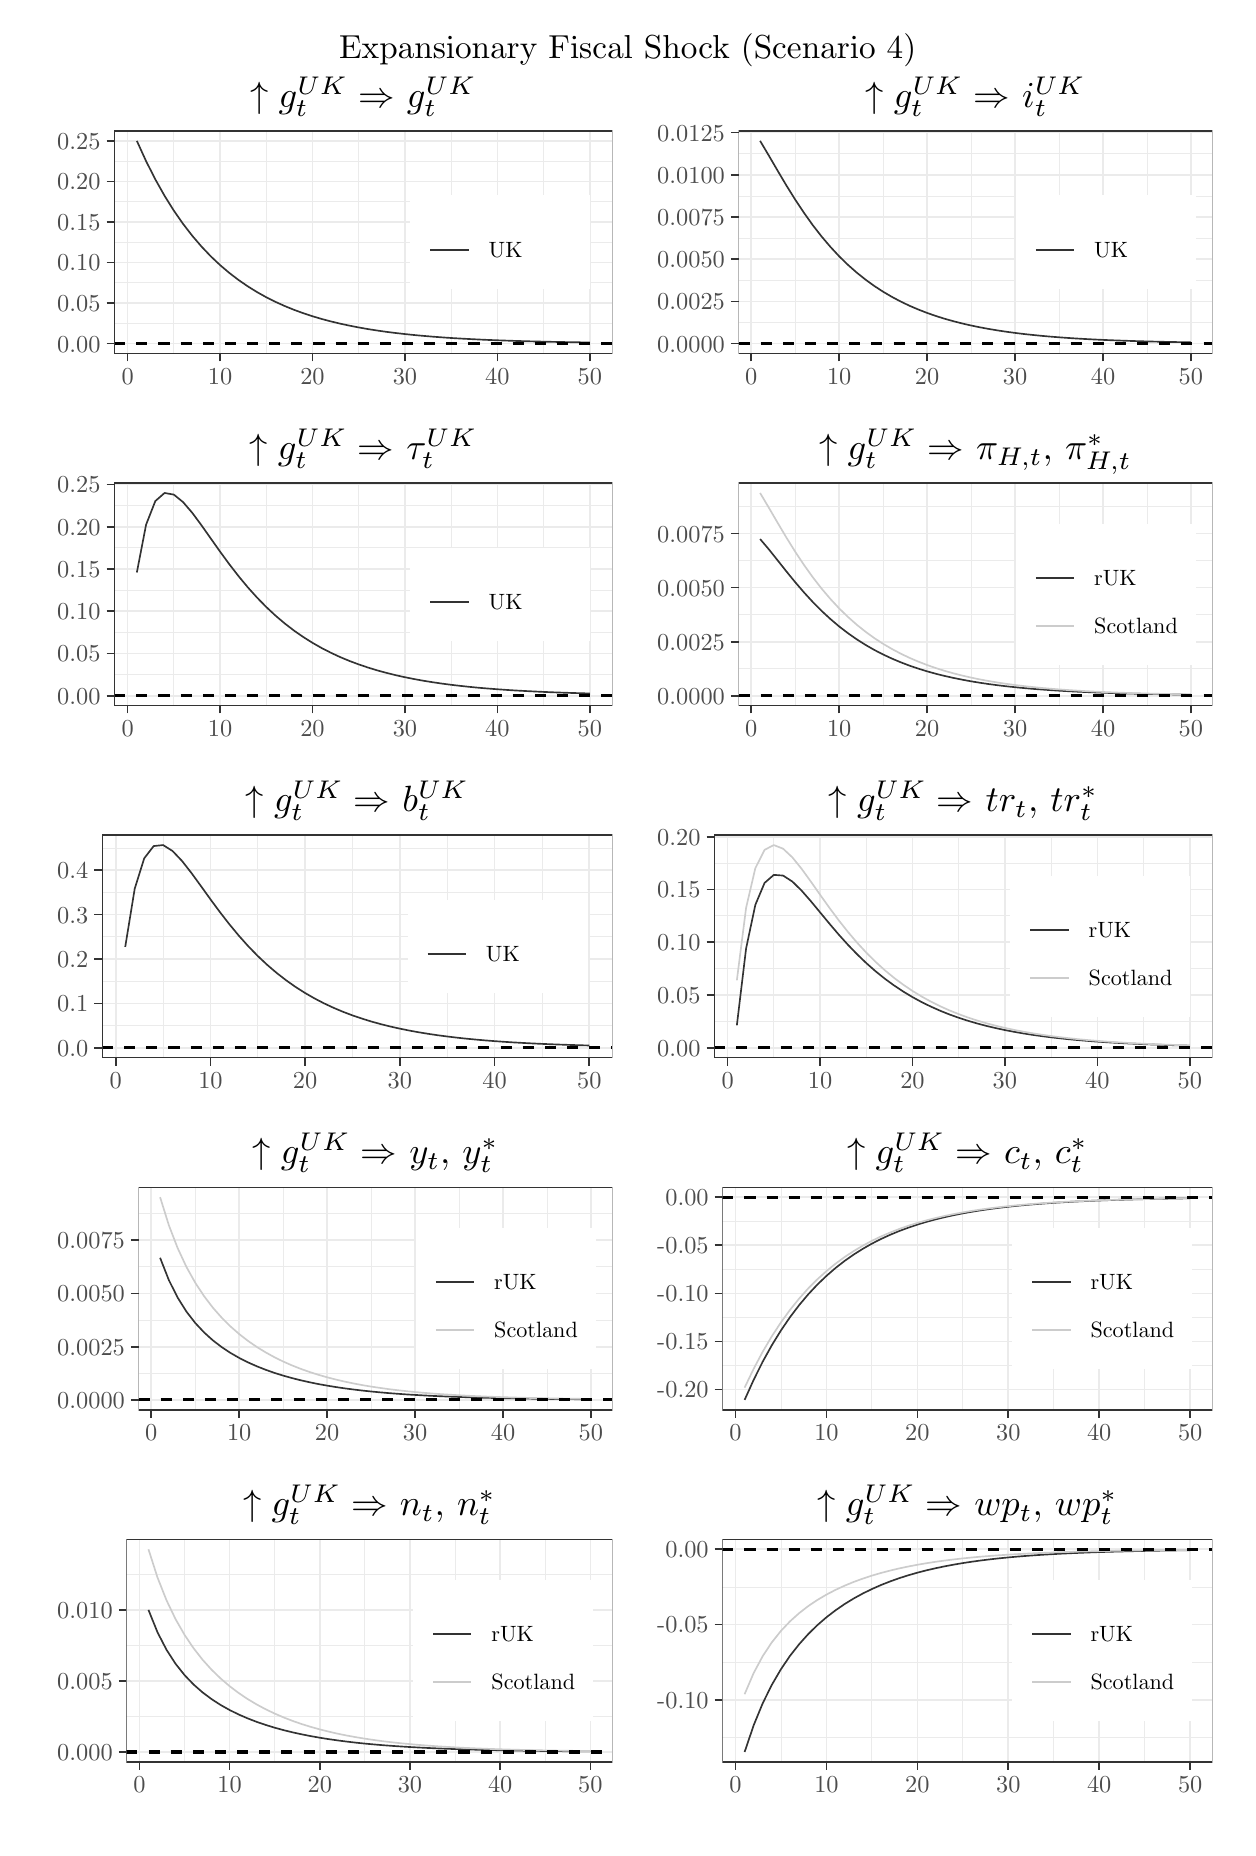
\begin{tikzpicture}[x=1pt,y=1pt]
\definecolor{fillColor}{RGB}{255,255,255}
\path[use as bounding box,fill=fillColor,fill opacity=0.00] (0,0) rectangle (433.62,650.43);
\begin{scope}
\path[clip] (  0.00,508.91) rectangle (216.81,636.14);
\definecolor{drawColor}{RGB}{255,255,255}
\definecolor{fillColor}{RGB}{255,255,255}

\path[draw=drawColor,line width= 0.6pt,line join=round,line cap=round,fill=fillColor] (  0.00,508.91) rectangle (216.81,636.14);
\end{scope}
\begin{scope}
\path[clip] ( 31.27,532.59) rectangle (211.31,613.18);
\definecolor{fillColor}{RGB}{255,255,255}

\path[fill=fillColor] ( 31.27,532.59) rectangle (211.31,613.18);
\definecolor{drawColor}{gray}{0.92}

\path[draw=drawColor,line width= 0.3pt,line join=round] ( 31.27,543.58) --
	(211.31,543.58);

\path[draw=drawColor,line width= 0.3pt,line join=round] ( 31.27,558.23) --
	(211.31,558.23);

\path[draw=drawColor,line width= 0.3pt,line join=round] ( 31.27,572.89) --
	(211.31,572.89);

\path[draw=drawColor,line width= 0.3pt,line join=round] ( 31.27,587.54) --
	(211.31,587.54);

\path[draw=drawColor,line width= 0.3pt,line join=round] ( 31.27,602.19) --
	(211.31,602.19);

\path[draw=drawColor,line width= 0.3pt,line join=round] ( 52.81,532.59) --
	( 52.81,613.18);

\path[draw=drawColor,line width= 0.3pt,line join=round] ( 86.22,532.59) --
	( 86.22,613.18);

\path[draw=drawColor,line width= 0.3pt,line join=round] (119.62,532.59) --
	(119.62,613.18);

\path[draw=drawColor,line width= 0.3pt,line join=round] (153.02,532.59) --
	(153.02,613.18);

\path[draw=drawColor,line width= 0.3pt,line join=round] (186.43,532.59) --
	(186.43,613.18);

\path[draw=drawColor,line width= 0.6pt,line join=round] ( 31.27,536.25) --
	(211.31,536.25);

\path[draw=drawColor,line width= 0.6pt,line join=round] ( 31.27,550.91) --
	(211.31,550.91);

\path[draw=drawColor,line width= 0.6pt,line join=round] ( 31.27,565.56) --
	(211.31,565.56);

\path[draw=drawColor,line width= 0.6pt,line join=round] ( 31.27,580.21) --
	(211.31,580.21);

\path[draw=drawColor,line width= 0.6pt,line join=round] ( 31.27,594.87) --
	(211.31,594.87);

\path[draw=drawColor,line width= 0.6pt,line join=round] ( 31.27,609.52) --
	(211.31,609.52);

\path[draw=drawColor,line width= 0.6pt,line join=round] ( 36.11,532.59) --
	( 36.11,613.18);

\path[draw=drawColor,line width= 0.6pt,line join=round] ( 69.52,532.59) --
	( 69.52,613.18);

\path[draw=drawColor,line width= 0.6pt,line join=round] (102.92,532.59) --
	(102.92,613.18);

\path[draw=drawColor,line width= 0.6pt,line join=round] (136.32,532.59) --
	(136.32,613.18);

\path[draw=drawColor,line width= 0.6pt,line join=round] (169.72,532.59) --
	(169.72,613.18);

\path[draw=drawColor,line width= 0.6pt,line join=round] (203.13,532.59) --
	(203.13,613.18);
\definecolor{drawColor}{gray}{0.20}

\path[draw=drawColor,line width= 0.6pt,line join=round] ( 39.45,609.52) --
	( 42.79,602.19) --
	( 46.13,595.60) --
	( 49.47,589.66) --
	( 52.81,584.32) --
	( 56.15,579.52) --
	( 59.50,575.19) --
	( 62.84,571.30) --
	( 66.18,567.79) --
	( 69.52,564.64) --
	( 72.86,561.80) --
	( 76.20,559.25) --
	( 79.54,556.95) --
	( 82.88,554.88) --
	( 86.22,553.01) --
	( 89.56,551.34) --
	( 92.90,549.83) --
	( 96.24,548.47) --
	( 99.58,547.25) --
	(102.92,546.15) --
	(106.26,545.16) --
	(109.60,544.27) --
	(112.94,543.47) --
	(116.28,542.75) --
	(119.62,542.10) --
	(122.96,541.51) --
	(126.30,540.99) --
	(129.64,540.51) --
	(132.98,540.09) --
	(136.32,539.71) --
	(139.66,539.36) --
	(143.00,539.05) --
	(146.34,538.77) --
	(149.68,538.52) --
	(153.02,538.29) --
	(156.36,538.09) --
	(159.70,537.91) --
	(163.04,537.74) --
	(166.38,537.59) --
	(169.72,537.46) --
	(173.06,537.34) --
	(176.40,537.23) --
	(179.74,537.13) --
	(183.08,537.04) --
	(186.43,536.97) --
	(189.77,536.89) --
	(193.11,536.83) --
	(196.45,536.77) --
	(199.79,536.72) --
	(203.13,536.67);
\definecolor{drawColor}{RGB}{0,0,0}

\path[draw=drawColor,line width= 1.1pt,dash pattern=on 4pt off 4pt ,line join=round] ( 31.27,536.25) -- (211.31,536.25);
\definecolor{drawColor}{gray}{0.20}

\path[draw=drawColor,line width= 0.6pt,line join=round,line cap=round] ( 31.27,532.59) rectangle (211.31,613.18);
\end{scope}
\begin{scope}
\path[clip] (  0.00,  0.00) rectangle (433.62,650.43);
\definecolor{drawColor}{gray}{0.30}

\node[text=drawColor,anchor=base east,inner sep=0pt, outer sep=0pt, scale=  0.88] at ( 26.32,533.22) {0.00};

\node[text=drawColor,anchor=base east,inner sep=0pt, outer sep=0pt, scale=  0.88] at ( 26.32,547.88) {0.05};

\node[text=drawColor,anchor=base east,inner sep=0pt, outer sep=0pt, scale=  0.88] at ( 26.32,562.53) {0.10};

\node[text=drawColor,anchor=base east,inner sep=0pt, outer sep=0pt, scale=  0.88] at ( 26.32,577.18) {0.15};

\node[text=drawColor,anchor=base east,inner sep=0pt, outer sep=0pt, scale=  0.88] at ( 26.32,591.83) {0.20};

\node[text=drawColor,anchor=base east,inner sep=0pt, outer sep=0pt, scale=  0.88] at ( 26.32,606.49) {0.25};
\end{scope}
\begin{scope}
\path[clip] (  0.00,  0.00) rectangle (433.62,650.43);
\definecolor{drawColor}{gray}{0.20}

\path[draw=drawColor,line width= 0.6pt,line join=round] ( 28.52,536.25) --
	( 31.27,536.25);

\path[draw=drawColor,line width= 0.6pt,line join=round] ( 28.52,550.91) --
	( 31.27,550.91);

\path[draw=drawColor,line width= 0.6pt,line join=round] ( 28.52,565.56) --
	( 31.27,565.56);

\path[draw=drawColor,line width= 0.6pt,line join=round] ( 28.52,580.21) --
	( 31.27,580.21);

\path[draw=drawColor,line width= 0.6pt,line join=round] ( 28.52,594.87) --
	( 31.27,594.87);

\path[draw=drawColor,line width= 0.6pt,line join=round] ( 28.52,609.52) --
	( 31.27,609.52);
\end{scope}
\begin{scope}
\path[clip] (  0.00,  0.00) rectangle (433.62,650.43);
\definecolor{drawColor}{gray}{0.20}

\path[draw=drawColor,line width= 0.6pt,line join=round] ( 36.11,529.84) --
	( 36.11,532.59);

\path[draw=drawColor,line width= 0.6pt,line join=round] ( 69.52,529.84) --
	( 69.52,532.59);

\path[draw=drawColor,line width= 0.6pt,line join=round] (102.92,529.84) --
	(102.92,532.59);

\path[draw=drawColor,line width= 0.6pt,line join=round] (136.32,529.84) --
	(136.32,532.59);

\path[draw=drawColor,line width= 0.6pt,line join=round] (169.72,529.84) --
	(169.72,532.59);

\path[draw=drawColor,line width= 0.6pt,line join=round] (203.13,529.84) --
	(203.13,532.59);
\end{scope}
\begin{scope}
\path[clip] (  0.00,  0.00) rectangle (433.62,650.43);
\definecolor{drawColor}{gray}{0.30}

\node[text=drawColor,anchor=base,inner sep=0pt, outer sep=0pt, scale=  0.88] at ( 36.11,521.58) {0};

\node[text=drawColor,anchor=base,inner sep=0pt, outer sep=0pt, scale=  0.88] at ( 69.52,521.58) {10};

\node[text=drawColor,anchor=base,inner sep=0pt, outer sep=0pt, scale=  0.88] at (102.92,521.58) {20};

\node[text=drawColor,anchor=base,inner sep=0pt, outer sep=0pt, scale=  0.88] at (136.32,521.58) {30};

\node[text=drawColor,anchor=base,inner sep=0pt, outer sep=0pt, scale=  0.88] at (169.72,521.58) {40};

\node[text=drawColor,anchor=base,inner sep=0pt, outer sep=0pt, scale=  0.88] at (203.13,521.58) {50};
\end{scope}
\begin{scope}
\path[clip] (  0.00,  0.00) rectangle (433.62,650.43);
\definecolor{fillColor}{RGB}{255,255,255}

\path[fill=fillColor] (138.26,555.96) rectangle (203.35,589.81);
\end{scope}
\begin{scope}
\path[clip] (  0.00,  0.00) rectangle (433.62,650.43);
\definecolor{fillColor}{RGB}{255,255,255}

\path[fill=fillColor] (143.76,561.46) rectangle (161.10,578.81);
\end{scope}
\begin{scope}
\path[clip] (  0.00,  0.00) rectangle (433.62,650.43);
\definecolor{drawColor}{gray}{0.20}

\path[draw=drawColor,line width= 0.6pt,line join=round] (145.49,570.14) -- (159.37,570.14);
\end{scope}
\begin{scope}
\path[clip] (  0.00,  0.00) rectangle (433.62,650.43);
\definecolor{drawColor}{RGB}{0,0,0}

\node[text=drawColor,anchor=base west,inner sep=0pt, outer sep=0pt, scale=  0.80] at (166.60,567.38) {UK};
\end{scope}
\begin{scope}
\path[clip] (  0.00,  0.00) rectangle (433.62,650.43);
\definecolor{drawColor}{RGB}{0,0,0}

\node[text=drawColor,anchor=base,inner sep=0pt, outer sep=0pt, scale=  1.32] at (121.29,621.55) {$\uparrow  g^{UK}_t \Rightarrow $ ${g^{UK}_t}$};
\end{scope}
\begin{scope}
\path[clip] (216.81,508.91) rectangle (433.62,636.14);
\definecolor{drawColor}{RGB}{255,255,255}
\definecolor{fillColor}{RGB}{255,255,255}

\path[draw=drawColor,line width= 0.6pt,line join=round,line cap=round,fill=fillColor] (216.81,508.91) rectangle (433.62,636.14);
\end{scope}
\begin{scope}
\path[clip] (256.88,532.59) rectangle (428.12,613.18);
\definecolor{fillColor}{RGB}{255,255,255}

\path[fill=fillColor] (256.88,532.59) rectangle (428.12,613.18);
\definecolor{drawColor}{gray}{0.92}

\path[draw=drawColor,line width= 0.3pt,line join=round] (256.88,543.88) --
	(428.12,543.88);

\path[draw=drawColor,line width= 0.3pt,line join=round] (256.88,559.12) --
	(428.12,559.12);

\path[draw=drawColor,line width= 0.3pt,line join=round] (256.88,574.37) --
	(428.12,574.37);

\path[draw=drawColor,line width= 0.3pt,line join=round] (256.88,589.62) --
	(428.12,589.62);

\path[draw=drawColor,line width= 0.3pt,line join=round] (256.88,604.86) --
	(428.12,604.86);

\path[draw=drawColor,line width= 0.3pt,line join=round] (277.37,532.59) --
	(277.37,613.18);

\path[draw=drawColor,line width= 0.3pt,line join=round] (309.14,532.59) --
	(309.14,613.18);

\path[draw=drawColor,line width= 0.3pt,line join=round] (340.91,532.59) --
	(340.91,613.18);

\path[draw=drawColor,line width= 0.3pt,line join=round] (372.68,532.59) --
	(372.68,613.18);

\path[draw=drawColor,line width= 0.3pt,line join=round] (404.45,532.59) --
	(404.45,613.18);

\path[draw=drawColor,line width= 0.6pt,line join=round] (256.88,536.25) --
	(428.12,536.25);

\path[draw=drawColor,line width= 0.6pt,line join=round] (256.88,551.50) --
	(428.12,551.50);

\path[draw=drawColor,line width= 0.6pt,line join=round] (256.88,566.75) --
	(428.12,566.75);

\path[draw=drawColor,line width= 0.6pt,line join=round] (256.88,581.99) --
	(428.12,581.99);

\path[draw=drawColor,line width= 0.6pt,line join=round] (256.88,597.24) --
	(428.12,597.24);

\path[draw=drawColor,line width= 0.6pt,line join=round] (256.88,612.49) --
	(428.12,612.49);

\path[draw=drawColor,line width= 0.6pt,line join=round] (261.48,532.59) --
	(261.48,613.18);

\path[draw=drawColor,line width= 0.6pt,line join=round] (293.25,532.59) --
	(293.25,613.18);

\path[draw=drawColor,line width= 0.6pt,line join=round] (325.03,532.59) --
	(325.03,613.18);

\path[draw=drawColor,line width= 0.6pt,line join=round] (356.80,532.59) --
	(356.80,613.18);

\path[draw=drawColor,line width= 0.6pt,line join=round] (388.57,532.59) --
	(388.57,613.18);

\path[draw=drawColor,line width= 0.6pt,line join=round] (420.34,532.59) --
	(420.34,613.18);
\definecolor{drawColor}{gray}{0.20}

\path[draw=drawColor,line width= 0.6pt,line join=round] (264.66,609.52) --
	(267.84,604.16) --
	(271.02,598.70) --
	(274.19,593.35) --
	(277.37,588.25) --
	(280.55,583.47) --
	(283.72,579.02) --
	(286.90,574.94) --
	(290.08,571.20) --
	(293.25,567.79) --
	(296.43,564.69) --
	(299.61,561.89) --
	(302.79,559.35) --
	(305.96,557.06) --
	(309.14,554.99) --
	(312.32,553.13) --
	(315.49,551.45) --
	(318.67,549.93) --
	(321.85,548.57) --
	(325.03,547.34) --
	(328.20,546.23) --
	(331.38,545.23) --
	(334.56,544.34) --
	(337.73,543.53) --
	(340.91,542.80) --
	(344.09,542.15) --
	(347.26,541.56) --
	(350.44,541.03) --
	(353.62,540.55) --
	(356.80,540.12) --
	(359.97,539.73) --
	(363.15,539.39) --
	(366.33,539.07) --
	(369.50,538.79) --
	(372.68,538.54) --
	(375.86,538.31) --
	(379.03,538.10) --
	(382.21,537.92) --
	(385.39,537.75) --
	(388.57,537.60) --
	(391.74,537.47) --
	(394.92,537.35) --
	(398.10,537.24) --
	(401.27,537.14) --
	(404.45,537.05) --
	(407.63,536.97) --
	(410.81,536.90) --
	(413.98,536.83) --
	(417.16,536.78) --
	(420.34,536.72);
\definecolor{drawColor}{RGB}{0,0,0}

\path[draw=drawColor,line width= 1.1pt,dash pattern=on 4pt off 4pt ,line join=round] (256.88,536.25) -- (428.12,536.25);
\definecolor{drawColor}{gray}{0.20}

\path[draw=drawColor,line width= 0.6pt,line join=round,line cap=round] (256.88,532.59) rectangle (428.12,613.18);
\end{scope}
\begin{scope}
\path[clip] (  0.00,  0.00) rectangle (433.62,650.43);
\definecolor{drawColor}{gray}{0.30}

\node[text=drawColor,anchor=base east,inner sep=0pt, outer sep=0pt, scale=  0.88] at (251.93,533.22) {0.0000};

\node[text=drawColor,anchor=base east,inner sep=0pt, outer sep=0pt, scale=  0.88] at (251.93,548.47) {0.0025};

\node[text=drawColor,anchor=base east,inner sep=0pt, outer sep=0pt, scale=  0.88] at (251.93,563.72) {0.0050};

\node[text=drawColor,anchor=base east,inner sep=0pt, outer sep=0pt, scale=  0.88] at (251.93,578.96) {0.0075};

\node[text=drawColor,anchor=base east,inner sep=0pt, outer sep=0pt, scale=  0.88] at (251.93,594.21) {0.0100};

\node[text=drawColor,anchor=base east,inner sep=0pt, outer sep=0pt, scale=  0.88] at (251.93,609.46) {0.0125};
\end{scope}
\begin{scope}
\path[clip] (  0.00,  0.00) rectangle (433.62,650.43);
\definecolor{drawColor}{gray}{0.20}

\path[draw=drawColor,line width= 0.6pt,line join=round] (254.13,536.25) --
	(256.88,536.25);

\path[draw=drawColor,line width= 0.6pt,line join=round] (254.13,551.50) --
	(256.88,551.50);

\path[draw=drawColor,line width= 0.6pt,line join=round] (254.13,566.75) --
	(256.88,566.75);

\path[draw=drawColor,line width= 0.6pt,line join=round] (254.13,581.99) --
	(256.88,581.99);

\path[draw=drawColor,line width= 0.6pt,line join=round] (254.13,597.24) --
	(256.88,597.24);

\path[draw=drawColor,line width= 0.6pt,line join=round] (254.13,612.49) --
	(256.88,612.49);
\end{scope}
\begin{scope}
\path[clip] (  0.00,  0.00) rectangle (433.62,650.43);
\definecolor{drawColor}{gray}{0.20}

\path[draw=drawColor,line width= 0.6pt,line join=round] (261.48,529.84) --
	(261.48,532.59);

\path[draw=drawColor,line width= 0.6pt,line join=round] (293.25,529.84) --
	(293.25,532.59);

\path[draw=drawColor,line width= 0.6pt,line join=round] (325.03,529.84) --
	(325.03,532.59);

\path[draw=drawColor,line width= 0.6pt,line join=round] (356.80,529.84) --
	(356.80,532.59);

\path[draw=drawColor,line width= 0.6pt,line join=round] (388.57,529.84) --
	(388.57,532.59);

\path[draw=drawColor,line width= 0.6pt,line join=round] (420.34,529.84) --
	(420.34,532.59);
\end{scope}
\begin{scope}
\path[clip] (  0.00,  0.00) rectangle (433.62,650.43);
\definecolor{drawColor}{gray}{0.30}

\node[text=drawColor,anchor=base,inner sep=0pt, outer sep=0pt, scale=  0.88] at (261.48,521.58) {0};

\node[text=drawColor,anchor=base,inner sep=0pt, outer sep=0pt, scale=  0.88] at (293.25,521.58) {10};

\node[text=drawColor,anchor=base,inner sep=0pt, outer sep=0pt, scale=  0.88] at (325.03,521.58) {20};

\node[text=drawColor,anchor=base,inner sep=0pt, outer sep=0pt, scale=  0.88] at (356.80,521.58) {30};

\node[text=drawColor,anchor=base,inner sep=0pt, outer sep=0pt, scale=  0.88] at (388.57,521.58) {40};

\node[text=drawColor,anchor=base,inner sep=0pt, outer sep=0pt, scale=  0.88] at (420.34,521.58) {50};
\end{scope}
\begin{scope}
\path[clip] (  0.00,  0.00) rectangle (433.62,650.43);
\definecolor{fillColor}{RGB}{255,255,255}

\path[fill=fillColor] (357.05,555.96) rectangle (422.14,589.81);
\end{scope}
\begin{scope}
\path[clip] (  0.00,  0.00) rectangle (433.62,650.43);
\definecolor{fillColor}{RGB}{255,255,255}

\path[fill=fillColor] (362.55,561.46) rectangle (379.89,578.81);
\end{scope}
\begin{scope}
\path[clip] (  0.00,  0.00) rectangle (433.62,650.43);
\definecolor{drawColor}{gray}{0.20}

\path[draw=drawColor,line width= 0.6pt,line join=round] (364.28,570.14) -- (378.16,570.14);
\end{scope}
\begin{scope}
\path[clip] (  0.00,  0.00) rectangle (433.62,650.43);
\definecolor{drawColor}{RGB}{0,0,0}

\node[text=drawColor,anchor=base west,inner sep=0pt, outer sep=0pt, scale=  0.80] at (385.39,567.38) {UK};
\end{scope}
\begin{scope}
\path[clip] (  0.00,  0.00) rectangle (433.62,650.43);
\definecolor{drawColor}{RGB}{0,0,0}

\node[text=drawColor,anchor=base,inner sep=0pt, outer sep=0pt, scale=  1.32] at (342.50,621.55) {$\uparrow  g^{UK}_t \Rightarrow $ ${i^{UK}_t}$};
\end{scope}
\begin{scope}
\path[clip] (  0.00,381.69) rectangle (216.81,508.91);
\definecolor{drawColor}{RGB}{255,255,255}
\definecolor{fillColor}{RGB}{255,255,255}

\path[draw=drawColor,line width= 0.6pt,line join=round,line cap=round,fill=fillColor] (  0.00,381.69) rectangle (216.81,508.91);
\end{scope}
\begin{scope}
\path[clip] ( 31.27,405.36) rectangle (211.31,485.95);
\definecolor{fillColor}{RGB}{255,255,255}

\path[fill=fillColor] ( 31.27,405.36) rectangle (211.31,485.95);
\definecolor{drawColor}{gray}{0.92}

\path[draw=drawColor,line width= 0.3pt,line join=round] ( 31.27,416.66) --
	(211.31,416.66);

\path[draw=drawColor,line width= 0.3pt,line join=round] ( 31.27,431.92) --
	(211.31,431.92);

\path[draw=drawColor,line width= 0.3pt,line join=round] ( 31.27,447.19) --
	(211.31,447.19);

\path[draw=drawColor,line width= 0.3pt,line join=round] ( 31.27,462.45) --
	(211.31,462.45);

\path[draw=drawColor,line width= 0.3pt,line join=round] ( 31.27,477.71) --
	(211.31,477.71);

\path[draw=drawColor,line width= 0.3pt,line join=round] ( 52.81,405.36) --
	( 52.81,485.95);

\path[draw=drawColor,line width= 0.3pt,line join=round] ( 86.22,405.36) --
	( 86.22,485.95);

\path[draw=drawColor,line width= 0.3pt,line join=round] (119.62,405.36) --
	(119.62,485.95);

\path[draw=drawColor,line width= 0.3pt,line join=round] (153.02,405.36) --
	(153.02,485.95);

\path[draw=drawColor,line width= 0.3pt,line join=round] (186.43,405.36) --
	(186.43,485.95);

\path[draw=drawColor,line width= 0.6pt,line join=round] ( 31.27,409.03) --
	(211.31,409.03);

\path[draw=drawColor,line width= 0.6pt,line join=round] ( 31.27,424.29) --
	(211.31,424.29);

\path[draw=drawColor,line width= 0.6pt,line join=round] ( 31.27,439.55) --
	(211.31,439.55);

\path[draw=drawColor,line width= 0.6pt,line join=round] ( 31.27,454.82) --
	(211.31,454.82);

\path[draw=drawColor,line width= 0.6pt,line join=round] ( 31.27,470.08) --
	(211.31,470.08);

\path[draw=drawColor,line width= 0.6pt,line join=round] ( 31.27,485.35) --
	(211.31,485.35);

\path[draw=drawColor,line width= 0.6pt,line join=round] ( 36.11,405.36) --
	( 36.11,485.95);

\path[draw=drawColor,line width= 0.6pt,line join=round] ( 69.52,405.36) --
	( 69.52,485.95);

\path[draw=drawColor,line width= 0.6pt,line join=round] (102.92,405.36) --
	(102.92,485.95);

\path[draw=drawColor,line width= 0.6pt,line join=round] (136.32,405.36) --
	(136.32,485.95);

\path[draw=drawColor,line width= 0.6pt,line join=round] (169.72,405.36) --
	(169.72,485.95);

\path[draw=drawColor,line width= 0.6pt,line join=round] (203.13,405.36) --
	(203.13,485.95);
\definecolor{drawColor}{gray}{0.20}

\path[draw=drawColor,line width= 0.6pt,line join=round] ( 39.45,453.56) --
	( 42.79,470.84) --
	( 46.13,479.37) --
	( 49.47,482.29) --
	( 52.81,481.70) --
	( 56.15,478.99) --
	( 59.50,475.08) --
	( 62.84,470.56) --
	( 66.18,465.82) --
	( 69.52,461.10) --
	( 72.86,456.54) --
	( 76.20,452.23) --
	( 79.54,448.20) --
	( 82.88,444.49) --
	( 86.22,441.08) --
	( 89.56,437.96) --
	( 92.90,435.13) --
	( 96.24,432.56) --
	( 99.58,430.24) --
	(102.92,428.14) --
	(106.26,426.24) --
	(109.60,424.53) --
	(112.94,422.98) --
	(116.28,421.59) --
	(119.62,420.34) --
	(122.96,419.21) --
	(126.30,418.19) --
	(129.64,417.28) --
	(132.98,416.45) --
	(136.32,415.71) --
	(139.66,415.04) --
	(143.00,414.44) --
	(146.34,413.90) --
	(149.68,413.41) --
	(153.02,412.97) --
	(156.36,412.58) --
	(159.70,412.22) --
	(163.04,411.90) --
	(166.38,411.62) --
	(169.72,411.36) --
	(173.06,411.12) --
	(176.40,410.91) --
	(179.74,410.73) --
	(183.08,410.56) --
	(186.43,410.40) --
	(189.77,410.26) --
	(193.11,410.14) --
	(196.45,410.03) --
	(199.79,409.93) --
	(203.13,409.84);
\definecolor{drawColor}{RGB}{0,0,0}

\path[draw=drawColor,line width= 1.1pt,dash pattern=on 4pt off 4pt ,line join=round] ( 31.27,409.03) -- (211.31,409.03);
\definecolor{drawColor}{gray}{0.20}

\path[draw=drawColor,line width= 0.6pt,line join=round,line cap=round] ( 31.27,405.36) rectangle (211.31,485.95);
\end{scope}
\begin{scope}
\path[clip] (  0.00,  0.00) rectangle (433.62,650.43);
\definecolor{drawColor}{gray}{0.30}

\node[text=drawColor,anchor=base east,inner sep=0pt, outer sep=0pt, scale=  0.88] at ( 26.32,406.00) {0.00};

\node[text=drawColor,anchor=base east,inner sep=0pt, outer sep=0pt, scale=  0.88] at ( 26.32,421.26) {0.05};

\node[text=drawColor,anchor=base east,inner sep=0pt, outer sep=0pt, scale=  0.88] at ( 26.32,436.52) {0.10};

\node[text=drawColor,anchor=base east,inner sep=0pt, outer sep=0pt, scale=  0.88] at ( 26.32,451.79) {0.15};

\node[text=drawColor,anchor=base east,inner sep=0pt, outer sep=0pt, scale=  0.88] at ( 26.32,467.05) {0.20};

\node[text=drawColor,anchor=base east,inner sep=0pt, outer sep=0pt, scale=  0.88] at ( 26.32,482.31) {0.25};
\end{scope}
\begin{scope}
\path[clip] (  0.00,  0.00) rectangle (433.62,650.43);
\definecolor{drawColor}{gray}{0.20}

\path[draw=drawColor,line width= 0.6pt,line join=round] ( 28.52,409.03) --
	( 31.27,409.03);

\path[draw=drawColor,line width= 0.6pt,line join=round] ( 28.52,424.29) --
	( 31.27,424.29);

\path[draw=drawColor,line width= 0.6pt,line join=round] ( 28.52,439.55) --
	( 31.27,439.55);

\path[draw=drawColor,line width= 0.6pt,line join=round] ( 28.52,454.82) --
	( 31.27,454.82);

\path[draw=drawColor,line width= 0.6pt,line join=round] ( 28.52,470.08) --
	( 31.27,470.08);

\path[draw=drawColor,line width= 0.6pt,line join=round] ( 28.52,485.35) --
	( 31.27,485.35);
\end{scope}
\begin{scope}
\path[clip] (  0.00,  0.00) rectangle (433.62,650.43);
\definecolor{drawColor}{gray}{0.20}

\path[draw=drawColor,line width= 0.6pt,line join=round] ( 36.11,402.61) --
	( 36.11,405.36);

\path[draw=drawColor,line width= 0.6pt,line join=round] ( 69.52,402.61) --
	( 69.52,405.36);

\path[draw=drawColor,line width= 0.6pt,line join=round] (102.92,402.61) --
	(102.92,405.36);

\path[draw=drawColor,line width= 0.6pt,line join=round] (136.32,402.61) --
	(136.32,405.36);

\path[draw=drawColor,line width= 0.6pt,line join=round] (169.72,402.61) --
	(169.72,405.36);

\path[draw=drawColor,line width= 0.6pt,line join=round] (203.13,402.61) --
	(203.13,405.36);
\end{scope}
\begin{scope}
\path[clip] (  0.00,  0.00) rectangle (433.62,650.43);
\definecolor{drawColor}{gray}{0.30}

\node[text=drawColor,anchor=base,inner sep=0pt, outer sep=0pt, scale=  0.88] at ( 36.11,394.35) {0};

\node[text=drawColor,anchor=base,inner sep=0pt, outer sep=0pt, scale=  0.88] at ( 69.52,394.35) {10};

\node[text=drawColor,anchor=base,inner sep=0pt, outer sep=0pt, scale=  0.88] at (102.92,394.35) {20};

\node[text=drawColor,anchor=base,inner sep=0pt, outer sep=0pt, scale=  0.88] at (136.32,394.35) {30};

\node[text=drawColor,anchor=base,inner sep=0pt, outer sep=0pt, scale=  0.88] at (169.72,394.35) {40};

\node[text=drawColor,anchor=base,inner sep=0pt, outer sep=0pt, scale=  0.88] at (203.13,394.35) {50};
\end{scope}
\begin{scope}
\path[clip] (  0.00,  0.00) rectangle (433.62,650.43);
\definecolor{fillColor}{RGB}{255,255,255}

\path[fill=fillColor] (138.26,428.74) rectangle (203.35,462.58);
\end{scope}
\begin{scope}
\path[clip] (  0.00,  0.00) rectangle (433.62,650.43);
\definecolor{fillColor}{RGB}{255,255,255}

\path[fill=fillColor] (143.76,434.24) rectangle (161.10,451.58);
\end{scope}
\begin{scope}
\path[clip] (  0.00,  0.00) rectangle (433.62,650.43);
\definecolor{drawColor}{gray}{0.20}

\path[draw=drawColor,line width= 0.6pt,line join=round] (145.49,442.91) -- (159.37,442.91);
\end{scope}
\begin{scope}
\path[clip] (  0.00,  0.00) rectangle (433.62,650.43);
\definecolor{drawColor}{RGB}{0,0,0}

\node[text=drawColor,anchor=base west,inner sep=0pt, outer sep=0pt, scale=  0.80] at (166.60,440.15) {UK};
\end{scope}
\begin{scope}
\path[clip] (  0.00,  0.00) rectangle (433.62,650.43);
\definecolor{drawColor}{RGB}{0,0,0}

\node[text=drawColor,anchor=base,inner sep=0pt, outer sep=0pt, scale=  1.32] at (121.29,494.32) {$\uparrow  g^{UK}_t \Rightarrow $ ${\tau^{UK}_t}$};
\end{scope}
\begin{scope}
\path[clip] (216.81,381.69) rectangle (433.62,508.91);
\definecolor{drawColor}{RGB}{255,255,255}
\definecolor{fillColor}{RGB}{255,255,255}

\path[draw=drawColor,line width= 0.6pt,line join=round,line cap=round,fill=fillColor] (216.81,381.69) rectangle (433.62,508.91);
\end{scope}
\begin{scope}
\path[clip] (256.88,405.36) rectangle (428.12,485.95);
\definecolor{fillColor}{RGB}{255,255,255}

\path[fill=fillColor] (256.88,405.36) rectangle (428.12,485.95);
\definecolor{drawColor}{gray}{0.92}

\path[draw=drawColor,line width= 0.3pt,line join=round] (256.88,418.79) --
	(428.12,418.79);

\path[draw=drawColor,line width= 0.3pt,line join=round] (256.88,438.32) --
	(428.12,438.32);

\path[draw=drawColor,line width= 0.3pt,line join=round] (256.88,457.84) --
	(428.12,457.84);

\path[draw=drawColor,line width= 0.3pt,line join=round] (256.88,477.37) --
	(428.12,477.37);

\path[draw=drawColor,line width= 0.3pt,line join=round] (277.37,405.36) --
	(277.37,485.95);

\path[draw=drawColor,line width= 0.3pt,line join=round] (309.14,405.36) --
	(309.14,485.95);

\path[draw=drawColor,line width= 0.3pt,line join=round] (340.91,405.36) --
	(340.91,485.95);

\path[draw=drawColor,line width= 0.3pt,line join=round] (372.68,405.36) --
	(372.68,485.95);

\path[draw=drawColor,line width= 0.3pt,line join=round] (404.45,405.36) --
	(404.45,485.95);

\path[draw=drawColor,line width= 0.6pt,line join=round] (256.88,409.03) --
	(428.12,409.03);

\path[draw=drawColor,line width= 0.6pt,line join=round] (256.88,428.55) --
	(428.12,428.55);

\path[draw=drawColor,line width= 0.6pt,line join=round] (256.88,448.08) --
	(428.12,448.08);

\path[draw=drawColor,line width= 0.6pt,line join=round] (256.88,467.60) --
	(428.12,467.60);

\path[draw=drawColor,line width= 0.6pt,line join=round] (261.48,405.36) --
	(261.48,485.95);

\path[draw=drawColor,line width= 0.6pt,line join=round] (293.25,405.36) --
	(293.25,485.95);

\path[draw=drawColor,line width= 0.6pt,line join=round] (325.03,405.36) --
	(325.03,485.95);

\path[draw=drawColor,line width= 0.6pt,line join=round] (356.80,405.36) --
	(356.80,485.95);

\path[draw=drawColor,line width= 0.6pt,line join=round] (388.57,405.36) --
	(388.57,485.95);

\path[draw=drawColor,line width= 0.6pt,line join=round] (420.34,405.36) --
	(420.34,485.95);
\definecolor{drawColor}{gray}{0.20}

\path[draw=drawColor,line width= 0.6pt,line join=round] (264.66,465.64) --
	(267.84,461.90) --
	(271.02,457.91) --
	(274.19,453.91) --
	(277.37,450.02) --
	(280.55,446.32) --
	(283.72,442.86) --
	(286.90,439.66) --
	(290.08,436.73) --
	(293.25,434.04) --
	(296.43,431.60) --
	(299.61,429.38) --
	(302.79,427.37) --
	(305.96,425.55) --
	(309.14,423.91) --
	(312.32,422.43) --
	(315.49,421.10) --
	(318.67,419.89) --
	(321.85,418.81) --
	(325.03,417.83) --
	(328.20,416.95) --
	(331.38,416.16) --
	(334.56,415.45) --
	(337.73,414.81) --
	(340.91,414.23) --
	(344.09,413.71) --
	(347.26,413.24) --
	(350.44,412.82) --
	(353.62,412.44) --
	(356.80,412.10) --
	(359.97,411.79) --
	(363.15,411.51) --
	(366.33,411.27) --
	(369.50,411.04) --
	(372.68,410.84) --
	(375.86,410.66) --
	(379.03,410.50) --
	(382.21,410.35) --
	(385.39,410.22) --
	(388.57,410.10) --
	(391.74,409.99) --
	(394.92,409.89) --
	(398.10,409.81) --
	(401.27,409.73) --
	(404.45,409.66) --
	(407.63,409.60) --
	(410.81,409.54) --
	(413.98,409.49) --
	(417.16,409.44) --
	(420.34,409.40);
\definecolor{drawColor}{gray}{0.80}

\path[draw=drawColor,line width= 0.6pt,line join=round] (264.66,482.29) --
	(267.84,476.93) --
	(271.02,471.47) --
	(274.19,466.13) --
	(277.37,461.03) --
	(280.55,456.24) --
	(283.72,451.80) --
	(286.90,447.71) --
	(290.08,443.97) --
	(293.25,440.56) --
	(296.43,437.47) --
	(299.61,434.66) --
	(302.79,432.12) --
	(305.96,429.83) --
	(309.14,427.76) --
	(312.32,425.90) --
	(315.49,424.22) --
	(318.67,422.70) --
	(321.85,421.34) --
	(325.03,420.11) --
	(328.20,419.00) --
	(331.38,418.00) --
	(334.56,417.11) --
	(337.73,416.30) --
	(340.91,415.57) --
	(344.09,414.92) --
	(347.26,414.33) --
	(350.44,413.80) --
	(353.62,413.32) --
	(356.80,412.89) --
	(359.97,412.51) --
	(363.15,412.16) --
	(366.33,411.84) --
	(369.50,411.56) --
	(372.68,411.31) --
	(375.86,411.08) --
	(379.03,410.88) --
	(382.21,410.69) --
	(385.39,410.52) --
	(388.57,410.37) --
	(391.74,410.24) --
	(394.92,410.12) --
	(398.10,410.01) --
	(401.27,409.91) --
	(404.45,409.82) --
	(407.63,409.74) --
	(410.81,409.67) --
	(413.98,409.61) --
	(417.16,409.55) --
	(420.34,409.50);
\definecolor{drawColor}{RGB}{0,0,0}

\path[draw=drawColor,line width= 1.1pt,dash pattern=on 4pt off 4pt ,line join=round] (256.88,409.03) -- (428.12,409.03);
\definecolor{drawColor}{gray}{0.20}

\path[draw=drawColor,line width= 0.6pt,line join=round,line cap=round] (256.88,405.36) rectangle (428.12,485.95);
\end{scope}
\begin{scope}
\path[clip] (  0.00,  0.00) rectangle (433.62,650.43);
\definecolor{drawColor}{gray}{0.30}

\node[text=drawColor,anchor=base east,inner sep=0pt, outer sep=0pt, scale=  0.88] at (251.93,406.00) {0.0000};

\node[text=drawColor,anchor=base east,inner sep=0pt, outer sep=0pt, scale=  0.88] at (251.93,425.52) {0.0025};

\node[text=drawColor,anchor=base east,inner sep=0pt, outer sep=0pt, scale=  0.88] at (251.93,445.05) {0.0050};

\node[text=drawColor,anchor=base east,inner sep=0pt, outer sep=0pt, scale=  0.88] at (251.93,464.57) {0.0075};
\end{scope}
\begin{scope}
\path[clip] (  0.00,  0.00) rectangle (433.62,650.43);
\definecolor{drawColor}{gray}{0.20}

\path[draw=drawColor,line width= 0.6pt,line join=round] (254.13,409.03) --
	(256.88,409.03);

\path[draw=drawColor,line width= 0.6pt,line join=round] (254.13,428.55) --
	(256.88,428.55);

\path[draw=drawColor,line width= 0.6pt,line join=round] (254.13,448.08) --
	(256.88,448.08);

\path[draw=drawColor,line width= 0.6pt,line join=round] (254.13,467.60) --
	(256.88,467.60);
\end{scope}
\begin{scope}
\path[clip] (  0.00,  0.00) rectangle (433.62,650.43);
\definecolor{drawColor}{gray}{0.20}

\path[draw=drawColor,line width= 0.6pt,line join=round] (261.48,402.61) --
	(261.48,405.36);

\path[draw=drawColor,line width= 0.6pt,line join=round] (293.25,402.61) --
	(293.25,405.36);

\path[draw=drawColor,line width= 0.6pt,line join=round] (325.03,402.61) --
	(325.03,405.36);

\path[draw=drawColor,line width= 0.6pt,line join=round] (356.80,402.61) --
	(356.80,405.36);

\path[draw=drawColor,line width= 0.6pt,line join=round] (388.57,402.61) --
	(388.57,405.36);

\path[draw=drawColor,line width= 0.6pt,line join=round] (420.34,402.61) --
	(420.34,405.36);
\end{scope}
\begin{scope}
\path[clip] (  0.00,  0.00) rectangle (433.62,650.43);
\definecolor{drawColor}{gray}{0.30}

\node[text=drawColor,anchor=base,inner sep=0pt, outer sep=0pt, scale=  0.88] at (261.48,394.35) {0};

\node[text=drawColor,anchor=base,inner sep=0pt, outer sep=0pt, scale=  0.88] at (293.25,394.35) {10};

\node[text=drawColor,anchor=base,inner sep=0pt, outer sep=0pt, scale=  0.88] at (325.03,394.35) {20};

\node[text=drawColor,anchor=base,inner sep=0pt, outer sep=0pt, scale=  0.88] at (356.80,394.35) {30};

\node[text=drawColor,anchor=base,inner sep=0pt, outer sep=0pt, scale=  0.88] at (388.57,394.35) {40};

\node[text=drawColor,anchor=base,inner sep=0pt, outer sep=0pt, scale=  0.88] at (420.34,394.35) {50};
\end{scope}
\begin{scope}
\path[clip] (  0.00,  0.00) rectangle (433.62,650.43);
\definecolor{fillColor}{RGB}{255,255,255}

\path[fill=fillColor] (357.05,420.06) rectangle (422.14,471.25);
\end{scope}
\begin{scope}
\path[clip] (  0.00,  0.00) rectangle (433.62,650.43);
\definecolor{fillColor}{RGB}{255,255,255}

\path[fill=fillColor] (362.55,442.91) rectangle (379.89,460.25);
\end{scope}
\begin{scope}
\path[clip] (  0.00,  0.00) rectangle (433.62,650.43);
\definecolor{drawColor}{gray}{0.20}

\path[draw=drawColor,line width= 0.6pt,line join=round] (364.28,451.58) -- (378.16,451.58);
\end{scope}
\begin{scope}
\path[clip] (  0.00,  0.00) rectangle (433.62,650.43);
\definecolor{fillColor}{RGB}{255,255,255}

\path[fill=fillColor] (362.55,425.56) rectangle (379.89,442.91);
\end{scope}
\begin{scope}
\path[clip] (  0.00,  0.00) rectangle (433.62,650.43);
\definecolor{drawColor}{gray}{0.80}

\path[draw=drawColor,line width= 0.6pt,line join=round] (364.28,434.24) -- (378.16,434.24);
\end{scope}
\begin{scope}
\path[clip] (  0.00,  0.00) rectangle (433.62,650.43);
\definecolor{drawColor}{RGB}{0,0,0}

\node[text=drawColor,anchor=base west,inner sep=0pt, outer sep=0pt, scale=  0.80] at (385.39,448.83) {rUK};
\end{scope}
\begin{scope}
\path[clip] (  0.00,  0.00) rectangle (433.62,650.43);
\definecolor{drawColor}{RGB}{0,0,0}

\node[text=drawColor,anchor=base west,inner sep=0pt, outer sep=0pt, scale=  0.80] at (385.39,431.48) {Scotland};
\end{scope}
\begin{scope}
\path[clip] (  0.00,  0.00) rectangle (433.62,650.43);
\definecolor{drawColor}{RGB}{0,0,0}

\node[text=drawColor,anchor=base,inner sep=0pt, outer sep=0pt, scale=  1.32] at (342.50,494.32) {$\uparrow  g^{UK}_t \Rightarrow $ ${\pi_{H,t}}$, ${\pi^*_{H,t}}$};
\end{scope}
\begin{scope}
\path[clip] (  0.00,254.46) rectangle (216.81,381.69);
\definecolor{drawColor}{RGB}{255,255,255}
\definecolor{fillColor}{RGB}{255,255,255}

\path[draw=drawColor,line width= 0.6pt,line join=round,line cap=round,fill=fillColor] (  0.00,254.46) rectangle (216.81,381.69);
\end{scope}
\begin{scope}
\path[clip] ( 26.87,278.13) rectangle (211.31,358.72);
\definecolor{fillColor}{RGB}{255,255,255}

\path[fill=fillColor] ( 26.87,278.13) rectangle (211.31,358.72);
\definecolor{drawColor}{gray}{0.92}

\path[draw=drawColor,line width= 0.3pt,line join=round] ( 26.87,289.82) --
	(211.31,289.82);

\path[draw=drawColor,line width= 0.3pt,line join=round] ( 26.87,305.86) --
	(211.31,305.86);

\path[draw=drawColor,line width= 0.3pt,line join=round] ( 26.87,321.91) --
	(211.31,321.91);

\path[draw=drawColor,line width= 0.3pt,line join=round] ( 26.87,337.95) --
	(211.31,337.95);

\path[draw=drawColor,line width= 0.3pt,line join=round] ( 26.87,354.00) --
	(211.31,354.00);

\path[draw=drawColor,line width= 0.3pt,line join=round] ( 48.94,278.13) --
	( 48.94,358.72);

\path[draw=drawColor,line width= 0.3pt,line join=round] ( 83.16,278.13) --
	( 83.16,358.72);

\path[draw=drawColor,line width= 0.3pt,line join=round] (117.38,278.13) --
	(117.38,358.72);

\path[draw=drawColor,line width= 0.3pt,line join=round] (151.60,278.13) --
	(151.60,358.72);

\path[draw=drawColor,line width= 0.3pt,line join=round] (185.82,278.13) --
	(185.82,358.72);

\path[draw=drawColor,line width= 0.6pt,line join=round] ( 26.87,281.80) --
	(211.31,281.80);

\path[draw=drawColor,line width= 0.6pt,line join=round] ( 26.87,297.84) --
	(211.31,297.84);

\path[draw=drawColor,line width= 0.6pt,line join=round] ( 26.87,313.89) --
	(211.31,313.89);

\path[draw=drawColor,line width= 0.6pt,line join=round] ( 26.87,329.93) --
	(211.31,329.93);

\path[draw=drawColor,line width= 0.6pt,line join=round] ( 26.87,345.97) --
	(211.31,345.97);

\path[draw=drawColor,line width= 0.6pt,line join=round] ( 31.83,278.13) --
	( 31.83,358.72);

\path[draw=drawColor,line width= 0.6pt,line join=round] ( 66.05,278.13) --
	( 66.05,358.72);

\path[draw=drawColor,line width= 0.6pt,line join=round] (100.27,278.13) --
	(100.27,358.72);

\path[draw=drawColor,line width= 0.6pt,line join=round] (134.49,278.13) --
	(134.49,358.72);

\path[draw=drawColor,line width= 0.6pt,line join=round] (168.71,278.13) --
	(168.71,358.72);

\path[draw=drawColor,line width= 0.6pt,line join=round] (202.93,278.13) --
	(202.93,358.72);
\definecolor{drawColor}{gray}{0.20}

\path[draw=drawColor,line width= 0.6pt,line join=round] ( 35.25,318.26) --
	( 38.68,339.29) --
	( 42.10,350.24) --
	( 45.52,354.70) --
	( 48.94,355.06) --
	( 52.36,352.91) --
	( 55.79,349.30) --
	( 59.21,344.92) --
	( 62.63,340.22) --
	( 66.05,335.46) --
	( 69.47,330.83) --
	( 72.90,326.42) --
	( 76.32,322.30) --
	( 79.74,318.47) --
	( 83.16,314.96) --
	( 86.58,311.75) --
	( 90.00,308.83) --
	( 93.43,306.17) --
	( 96.85,303.76) --
	(100.27,301.59) --
	(103.69,299.63) --
	(107.11,297.85) --
	(110.54,296.25) --
	(113.96,294.81) --
	(117.38,293.51) --
	(120.80,292.35) --
	(124.22,291.29) --
	(127.65,290.34) --
	(131.07,289.49) --
	(134.49,288.72) --
	(137.91,288.03) --
	(141.33,287.41) --
	(144.75,286.85) --
	(148.18,286.34) --
	(151.60,285.89) --
	(155.02,285.48) --
	(158.44,285.11) --
	(161.86,284.78) --
	(165.29,284.48) --
	(168.71,284.21) --
	(172.13,283.97) --
	(175.55,283.75) --
	(178.97,283.56) --
	(182.40,283.38) --
	(185.82,283.22) --
	(189.24,283.08) --
	(192.66,282.95) --
	(196.08,282.84) --
	(199.50,282.73) --
	(202.93,282.64);
\definecolor{drawColor}{RGB}{0,0,0}

\path[draw=drawColor,line width= 1.1pt,dash pattern=on 4pt off 4pt ,line join=round] ( 26.87,281.80) -- (211.31,281.80);
\definecolor{drawColor}{gray}{0.20}

\path[draw=drawColor,line width= 0.6pt,line join=round,line cap=round] ( 26.87,278.13) rectangle (211.31,358.72);
\end{scope}
\begin{scope}
\path[clip] (  0.00,  0.00) rectangle (433.62,650.43);
\definecolor{drawColor}{gray}{0.30}

\node[text=drawColor,anchor=base east,inner sep=0pt, outer sep=0pt, scale=  0.88] at ( 21.92,278.77) {0.0};

\node[text=drawColor,anchor=base east,inner sep=0pt, outer sep=0pt, scale=  0.88] at ( 21.92,294.81) {0.1};

\node[text=drawColor,anchor=base east,inner sep=0pt, outer sep=0pt, scale=  0.88] at ( 21.92,310.86) {0.2};

\node[text=drawColor,anchor=base east,inner sep=0pt, outer sep=0pt, scale=  0.88] at ( 21.92,326.90) {0.3};

\node[text=drawColor,anchor=base east,inner sep=0pt, outer sep=0pt, scale=  0.88] at ( 21.92,342.94) {0.4};
\end{scope}
\begin{scope}
\path[clip] (  0.00,  0.00) rectangle (433.62,650.43);
\definecolor{drawColor}{gray}{0.20}

\path[draw=drawColor,line width= 0.6pt,line join=round] ( 24.12,281.80) --
	( 26.87,281.80);

\path[draw=drawColor,line width= 0.6pt,line join=round] ( 24.12,297.84) --
	( 26.87,297.84);

\path[draw=drawColor,line width= 0.6pt,line join=round] ( 24.12,313.89) --
	( 26.87,313.89);

\path[draw=drawColor,line width= 0.6pt,line join=round] ( 24.12,329.93) --
	( 26.87,329.93);

\path[draw=drawColor,line width= 0.6pt,line join=round] ( 24.12,345.97) --
	( 26.87,345.97);
\end{scope}
\begin{scope}
\path[clip] (  0.00,  0.00) rectangle (433.62,650.43);
\definecolor{drawColor}{gray}{0.20}

\path[draw=drawColor,line width= 0.6pt,line join=round] ( 31.83,275.38) --
	( 31.83,278.13);

\path[draw=drawColor,line width= 0.6pt,line join=round] ( 66.05,275.38) --
	( 66.05,278.13);

\path[draw=drawColor,line width= 0.6pt,line join=round] (100.27,275.38) --
	(100.27,278.13);

\path[draw=drawColor,line width= 0.6pt,line join=round] (134.49,275.38) --
	(134.49,278.13);

\path[draw=drawColor,line width= 0.6pt,line join=round] (168.71,275.38) --
	(168.71,278.13);

\path[draw=drawColor,line width= 0.6pt,line join=round] (202.93,275.38) --
	(202.93,278.13);
\end{scope}
\begin{scope}
\path[clip] (  0.00,  0.00) rectangle (433.62,650.43);
\definecolor{drawColor}{gray}{0.30}

\node[text=drawColor,anchor=base,inner sep=0pt, outer sep=0pt, scale=  0.88] at ( 31.83,267.12) {0};

\node[text=drawColor,anchor=base,inner sep=0pt, outer sep=0pt, scale=  0.88] at ( 66.05,267.12) {10};

\node[text=drawColor,anchor=base,inner sep=0pt, outer sep=0pt, scale=  0.88] at (100.27,267.12) {20};

\node[text=drawColor,anchor=base,inner sep=0pt, outer sep=0pt, scale=  0.88] at (134.49,267.12) {30};

\node[text=drawColor,anchor=base,inner sep=0pt, outer sep=0pt, scale=  0.88] at (168.71,267.12) {40};

\node[text=drawColor,anchor=base,inner sep=0pt, outer sep=0pt, scale=  0.88] at (202.93,267.12) {50};
\end{scope}
\begin{scope}
\path[clip] (  0.00,  0.00) rectangle (433.62,650.43);
\definecolor{fillColor}{RGB}{255,255,255}

\path[fill=fillColor] (137.27,301.51) rectangle (202.36,335.35);
\end{scope}
\begin{scope}
\path[clip] (  0.00,  0.00) rectangle (433.62,650.43);
\definecolor{fillColor}{RGB}{255,255,255}

\path[fill=fillColor] (142.77,307.01) rectangle (160.11,324.35);
\end{scope}
\begin{scope}
\path[clip] (  0.00,  0.00) rectangle (433.62,650.43);
\definecolor{drawColor}{gray}{0.20}

\path[draw=drawColor,line width= 0.6pt,line join=round] (144.50,315.68) -- (158.38,315.68);
\end{scope}
\begin{scope}
\path[clip] (  0.00,  0.00) rectangle (433.62,650.43);
\definecolor{drawColor}{RGB}{0,0,0}

\node[text=drawColor,anchor=base west,inner sep=0pt, outer sep=0pt, scale=  0.80] at (165.61,312.92) {UK};
\end{scope}
\begin{scope}
\path[clip] (  0.00,  0.00) rectangle (433.62,650.43);
\definecolor{drawColor}{RGB}{0,0,0}

\node[text=drawColor,anchor=base,inner sep=0pt, outer sep=0pt, scale=  1.32] at (119.09,367.09) {$\uparrow  g^{UK}_t \Rightarrow $ ${b^{UK}_t}$};
\end{scope}
\begin{scope}
\path[clip] (216.81,254.46) rectangle (433.62,381.69);
\definecolor{drawColor}{RGB}{255,255,255}
\definecolor{fillColor}{RGB}{255,255,255}

\path[draw=drawColor,line width= 0.6pt,line join=round,line cap=round,fill=fillColor] (216.81,254.46) rectangle (433.62,381.69);
\end{scope}
\begin{scope}
\path[clip] (248.08,278.13) rectangle (428.12,358.72);
\definecolor{fillColor}{RGB}{255,255,255}

\path[fill=fillColor] (248.08,278.13) rectangle (428.12,358.72);
\definecolor{drawColor}{gray}{0.92}

\path[draw=drawColor,line width= 0.3pt,line join=round] (248.08,291.33) --
	(428.12,291.33);

\path[draw=drawColor,line width= 0.3pt,line join=round] (248.08,310.39) --
	(428.12,310.39);

\path[draw=drawColor,line width= 0.3pt,line join=round] (248.08,329.46) --
	(428.12,329.46);

\path[draw=drawColor,line width= 0.3pt,line join=round] (248.08,348.52) --
	(428.12,348.52);

\path[draw=drawColor,line width= 0.3pt,line join=round] (269.62,278.13) --
	(269.62,358.72);

\path[draw=drawColor,line width= 0.3pt,line join=round] (303.03,278.13) --
	(303.03,358.72);

\path[draw=drawColor,line width= 0.3pt,line join=round] (336.43,278.13) --
	(336.43,358.72);

\path[draw=drawColor,line width= 0.3pt,line join=round] (369.83,278.13) --
	(369.83,358.72);

\path[draw=drawColor,line width= 0.3pt,line join=round] (403.24,278.13) --
	(403.24,358.72);

\path[draw=drawColor,line width= 0.6pt,line join=round] (248.08,281.80) --
	(428.12,281.80);

\path[draw=drawColor,line width= 0.6pt,line join=round] (248.08,300.86) --
	(428.12,300.86);

\path[draw=drawColor,line width= 0.6pt,line join=round] (248.08,319.92) --
	(428.12,319.92);

\path[draw=drawColor,line width= 0.6pt,line join=round] (248.08,338.99) --
	(428.12,338.99);

\path[draw=drawColor,line width= 0.6pt,line join=round] (248.08,358.05) --
	(428.12,358.05);

\path[draw=drawColor,line width= 0.6pt,line join=round] (252.92,278.13) --
	(252.92,358.72);

\path[draw=drawColor,line width= 0.6pt,line join=round] (286.33,278.13) --
	(286.33,358.72);

\path[draw=drawColor,line width= 0.6pt,line join=round] (319.73,278.13) --
	(319.73,358.72);

\path[draw=drawColor,line width= 0.6pt,line join=round] (353.13,278.13) --
	(353.13,358.72);

\path[draw=drawColor,line width= 0.6pt,line join=round] (386.53,278.13) --
	(386.53,358.72);

\path[draw=drawColor,line width= 0.6pt,line join=round] (419.94,278.13) --
	(419.94,358.72);
\definecolor{drawColor}{gray}{0.20}

\path[draw=drawColor,line width= 0.6pt,line join=round] (256.26,289.93) --
	(259.60,317.70) --
	(262.94,333.46) --
	(266.28,341.39) --
	(269.62,344.29) --
	(272.96,344.04) --
	(276.31,341.88) --
	(279.65,338.61) --
	(282.99,334.79) --
	(286.33,330.75) --
	(289.67,326.71) --
	(293.01,322.79) --
	(296.35,319.08) --
	(299.69,315.62) --
	(303.03,312.41) --
	(306.37,309.47) --
	(309.71,306.79) --
	(313.05,304.34) --
	(316.39,302.13) --
	(319.73,300.12) --
	(323.07,298.30) --
	(326.41,296.67) --
	(329.75,295.19) --
	(333.09,293.85) --
	(336.43,292.65) --
	(339.77,291.57) --
	(343.11,290.59) --
	(346.45,289.71) --
	(349.79,288.92) --
	(353.13,288.21) --
	(356.47,287.57) --
	(359.81,286.99) --
	(363.15,286.47) --
	(366.49,286.01) --
	(369.83,285.59) --
	(373.17,285.21) --
	(376.51,284.87) --
	(379.85,284.56) --
	(383.19,284.28) --
	(386.53,284.03) --
	(389.87,283.81) --
	(393.21,283.61) --
	(396.55,283.43) --
	(399.89,283.27) --
	(403.24,283.12) --
	(406.58,282.99) --
	(409.92,282.87) --
	(413.26,282.76) --
	(416.60,282.66) --
	(419.94,282.58);
\definecolor{drawColor}{gray}{0.80}

\path[draw=drawColor,line width= 0.6pt,line join=round] (256.26,306.19) --
	(259.60,332.39) --
	(262.94,346.71) --
	(266.28,353.34) --
	(269.62,355.06) --
	(272.96,353.75) --
	(276.31,350.62) --
	(279.65,346.49) --
	(282.99,341.88) --
	(286.33,337.13) --
	(289.67,332.45) --
	(293.01,327.96) --
	(296.35,323.74) --
	(299.69,319.81) --
	(303.03,316.19) --
	(306.37,312.87) --
	(309.71,309.84) --
	(313.05,307.09) --
	(316.39,304.60) --
	(319.73,302.35) --
	(323.07,300.31) --
	(326.41,298.47) --
	(329.75,296.81) --
	(333.09,295.31) --
	(336.43,293.97) --
	(339.77,292.75) --
	(343.11,291.66) --
	(346.45,290.67) --
	(349.79,289.79) --
	(353.13,288.99) --
	(356.47,288.27) --
	(359.81,287.62) --
	(363.15,287.04) --
	(366.49,286.52) --
	(369.83,286.04) --
	(373.17,285.62) --
	(376.51,285.24) --
	(379.85,284.89) --
	(383.19,284.58) --
	(386.53,284.31) --
	(389.87,284.05) --
	(393.21,283.83) --
	(396.55,283.63) --
	(399.89,283.44) --
	(403.24,283.28) --
	(406.58,283.13) --
	(409.92,283.00) --
	(413.26,282.88) --
	(416.60,282.77) --
	(419.94,282.67);
\definecolor{drawColor}{RGB}{0,0,0}

\path[draw=drawColor,line width= 1.1pt,dash pattern=on 4pt off 4pt ,line join=round] (248.08,281.80) -- (428.12,281.80);
\definecolor{drawColor}{gray}{0.20}

\path[draw=drawColor,line width= 0.6pt,line join=round,line cap=round] (248.08,278.13) rectangle (428.12,358.72);
\end{scope}
\begin{scope}
\path[clip] (  0.00,  0.00) rectangle (433.62,650.43);
\definecolor{drawColor}{gray}{0.30}

\node[text=drawColor,anchor=base east,inner sep=0pt, outer sep=0pt, scale=  0.88] at (243.13,278.77) {0.00};

\node[text=drawColor,anchor=base east,inner sep=0pt, outer sep=0pt, scale=  0.88] at (243.13,297.83) {0.05};

\node[text=drawColor,anchor=base east,inner sep=0pt, outer sep=0pt, scale=  0.88] at (243.13,316.89) {0.10};

\node[text=drawColor,anchor=base east,inner sep=0pt, outer sep=0pt, scale=  0.88] at (243.13,335.96) {0.15};

\node[text=drawColor,anchor=base east,inner sep=0pt, outer sep=0pt, scale=  0.88] at (243.13,355.02) {0.20};
\end{scope}
\begin{scope}
\path[clip] (  0.00,  0.00) rectangle (433.62,650.43);
\definecolor{drawColor}{gray}{0.20}

\path[draw=drawColor,line width= 0.6pt,line join=round] (245.33,281.80) --
	(248.08,281.80);

\path[draw=drawColor,line width= 0.6pt,line join=round] (245.33,300.86) --
	(248.08,300.86);

\path[draw=drawColor,line width= 0.6pt,line join=round] (245.33,319.92) --
	(248.08,319.92);

\path[draw=drawColor,line width= 0.6pt,line join=round] (245.33,338.99) --
	(248.08,338.99);

\path[draw=drawColor,line width= 0.6pt,line join=round] (245.33,358.05) --
	(248.08,358.05);
\end{scope}
\begin{scope}
\path[clip] (  0.00,  0.00) rectangle (433.62,650.43);
\definecolor{drawColor}{gray}{0.20}

\path[draw=drawColor,line width= 0.6pt,line join=round] (252.92,275.38) --
	(252.92,278.13);

\path[draw=drawColor,line width= 0.6pt,line join=round] (286.33,275.38) --
	(286.33,278.13);

\path[draw=drawColor,line width= 0.6pt,line join=round] (319.73,275.38) --
	(319.73,278.13);

\path[draw=drawColor,line width= 0.6pt,line join=round] (353.13,275.38) --
	(353.13,278.13);

\path[draw=drawColor,line width= 0.6pt,line join=round] (386.53,275.38) --
	(386.53,278.13);

\path[draw=drawColor,line width= 0.6pt,line join=round] (419.94,275.38) --
	(419.94,278.13);
\end{scope}
\begin{scope}
\path[clip] (  0.00,  0.00) rectangle (433.62,650.43);
\definecolor{drawColor}{gray}{0.30}

\node[text=drawColor,anchor=base,inner sep=0pt, outer sep=0pt, scale=  0.88] at (252.92,267.12) {0};

\node[text=drawColor,anchor=base,inner sep=0pt, outer sep=0pt, scale=  0.88] at (286.33,267.12) {10};

\node[text=drawColor,anchor=base,inner sep=0pt, outer sep=0pt, scale=  0.88] at (319.73,267.12) {20};

\node[text=drawColor,anchor=base,inner sep=0pt, outer sep=0pt, scale=  0.88] at (353.13,267.12) {30};

\node[text=drawColor,anchor=base,inner sep=0pt, outer sep=0pt, scale=  0.88] at (386.53,267.12) {40};

\node[text=drawColor,anchor=base,inner sep=0pt, outer sep=0pt, scale=  0.88] at (419.94,267.12) {50};
\end{scope}
\begin{scope}
\path[clip] (  0.00,  0.00) rectangle (433.62,650.43);
\definecolor{fillColor}{RGB}{255,255,255}

\path[fill=fillColor] (355.07,292.83) rectangle (420.16,344.02);
\end{scope}
\begin{scope}
\path[clip] (  0.00,  0.00) rectangle (433.62,650.43);
\definecolor{fillColor}{RGB}{255,255,255}

\path[fill=fillColor] (360.57,315.68) rectangle (377.91,333.02);
\end{scope}
\begin{scope}
\path[clip] (  0.00,  0.00) rectangle (433.62,650.43);
\definecolor{drawColor}{gray}{0.20}

\path[draw=drawColor,line width= 0.6pt,line join=round] (362.30,324.35) -- (376.18,324.35);
\end{scope}
\begin{scope}
\path[clip] (  0.00,  0.00) rectangle (433.62,650.43);
\definecolor{fillColor}{RGB}{255,255,255}

\path[fill=fillColor] (360.57,298.33) rectangle (377.91,315.68);
\end{scope}
\begin{scope}
\path[clip] (  0.00,  0.00) rectangle (433.62,650.43);
\definecolor{drawColor}{gray}{0.80}

\path[draw=drawColor,line width= 0.6pt,line join=round] (362.30,307.01) -- (376.18,307.01);
\end{scope}
\begin{scope}
\path[clip] (  0.00,  0.00) rectangle (433.62,650.43);
\definecolor{drawColor}{RGB}{0,0,0}

\node[text=drawColor,anchor=base west,inner sep=0pt, outer sep=0pt, scale=  0.80] at (383.41,321.60) {rUK};
\end{scope}
\begin{scope}
\path[clip] (  0.00,  0.00) rectangle (433.62,650.43);
\definecolor{drawColor}{RGB}{0,0,0}

\node[text=drawColor,anchor=base west,inner sep=0pt, outer sep=0pt, scale=  0.80] at (383.41,304.25) {Scotland};
\end{scope}
\begin{scope}
\path[clip] (  0.00,  0.00) rectangle (433.62,650.43);
\definecolor{drawColor}{RGB}{0,0,0}

\node[text=drawColor,anchor=base,inner sep=0pt, outer sep=0pt, scale=  1.32] at (338.10,367.09) {$\uparrow  g^{UK}_t \Rightarrow $ ${tr_t}$, ${tr^*_t}$};
\end{scope}
\begin{scope}
\path[clip] (  0.00,127.23) rectangle (216.81,254.46);
\definecolor{drawColor}{RGB}{255,255,255}
\definecolor{fillColor}{RGB}{255,255,255}

\path[draw=drawColor,line width= 0.6pt,line join=round,line cap=round,fill=fillColor] (  0.00,127.23) rectangle (216.81,254.46);
\end{scope}
\begin{scope}
\path[clip] ( 40.07,150.91) rectangle (211.31,231.50);
\definecolor{fillColor}{RGB}{255,255,255}

\path[fill=fillColor] ( 40.07,150.91) rectangle (211.31,231.50);
\definecolor{drawColor}{gray}{0.92}

\path[draw=drawColor,line width= 0.3pt,line join=round] ( 40.07,164.19) --
	(211.31,164.19);

\path[draw=drawColor,line width= 0.3pt,line join=round] ( 40.07,183.42) --
	(211.31,183.42);

\path[draw=drawColor,line width= 0.3pt,line join=round] ( 40.07,202.66) --
	(211.31,202.66);

\path[draw=drawColor,line width= 0.3pt,line join=round] ( 40.07,221.89) --
	(211.31,221.89);

\path[draw=drawColor,line width= 0.3pt,line join=round] ( 60.56,150.91) --
	( 60.56,231.50);

\path[draw=drawColor,line width= 0.3pt,line join=round] ( 92.33,150.91) --
	( 92.33,231.50);

\path[draw=drawColor,line width= 0.3pt,line join=round] (124.10,150.91) --
	(124.10,231.50);

\path[draw=drawColor,line width= 0.3pt,line join=round] (155.87,150.91) --
	(155.87,231.50);

\path[draw=drawColor,line width= 0.3pt,line join=round] (187.64,150.91) --
	(187.64,231.50);

\path[draw=drawColor,line width= 0.6pt,line join=round] ( 40.07,154.57) --
	(211.31,154.57);

\path[draw=drawColor,line width= 0.6pt,line join=round] ( 40.07,173.80) --
	(211.31,173.80);

\path[draw=drawColor,line width= 0.6pt,line join=round] ( 40.07,193.04) --
	(211.31,193.04);

\path[draw=drawColor,line width= 0.6pt,line join=round] ( 40.07,212.27) --
	(211.31,212.27);

\path[draw=drawColor,line width= 0.6pt,line join=round] ( 44.67,150.91) --
	( 44.67,231.50);

\path[draw=drawColor,line width= 0.6pt,line join=round] ( 76.44,150.91) --
	( 76.44,231.50);

\path[draw=drawColor,line width= 0.6pt,line join=round] (108.22,150.91) --
	(108.22,231.50);

\path[draw=drawColor,line width= 0.6pt,line join=round] (139.99,150.91) --
	(139.99,231.50);

\path[draw=drawColor,line width= 0.6pt,line join=round] (171.76,150.91) --
	(171.76,231.50);

\path[draw=drawColor,line width= 0.6pt,line join=round] (203.53,150.91) --
	(203.53,231.50);
\definecolor{drawColor}{gray}{0.20}

\path[draw=drawColor,line width= 0.6pt,line join=round] ( 47.85,205.92) --
	( 51.03,197.83) --
	( 54.21,191.51) --
	( 57.38,186.46) --
	( 60.56,182.36) --
	( 63.74,178.96) --
	( 66.91,176.10) --
	( 70.09,173.67) --
	( 73.27,171.56) --
	( 76.44,169.74) --
	( 79.62,168.13) --
	( 82.80,166.72) --
	( 85.98,165.46) --
	( 89.15,164.34) --
	( 92.33,163.35) --
	( 95.51,162.46) --
	( 98.68,161.66) --
	(101.86,160.95) --
	(105.04,160.30) --
	(108.22,159.73) --
	(111.39,159.21) --
	(114.57,158.74) --
	(117.75,158.33) --
	(120.92,157.95) --
	(124.10,157.61) --
	(127.28,157.31) --
	(130.45,157.03) --
	(133.63,156.79) --
	(136.81,156.56) --
	(139.99,156.37) --
	(143.16,156.19) --
	(146.34,156.02) --
	(149.52,155.88) --
	(152.69,155.75) --
	(155.87,155.63) --
	(159.05,155.52) --
	(162.22,155.43) --
	(165.40,155.34) --
	(168.58,155.26) --
	(171.76,155.20) --
	(174.93,155.13) --
	(178.11,155.08) --
	(181.29,155.03) --
	(184.46,154.98) --
	(187.64,154.94) --
	(190.82,154.90) --
	(194.00,154.87) --
	(197.17,154.84) --
	(200.35,154.81) --
	(203.53,154.79);
\definecolor{drawColor}{gray}{0.80}

\path[draw=drawColor,line width= 0.6pt,line join=round] ( 47.85,227.83) --
	( 51.03,217.64) --
	( 54.21,209.39) --
	( 57.38,202.59) --
	( 60.56,196.90) --
	( 63.74,192.07) --
	( 66.91,187.91) --
	( 70.09,184.30) --
	( 73.27,181.14) --
	( 76.44,178.36) --
	( 79.62,175.89) --
	( 82.80,173.70) --
	( 85.98,171.75) --
	( 89.15,170.01) --
	( 92.33,168.44) --
	( 95.51,167.04) --
	( 98.68,165.79) --
	(101.86,164.66) --
	(105.04,163.65) --
	(108.22,162.74) --
	(111.39,161.92) --
	(114.57,161.18) --
	(117.75,160.52) --
	(120.92,159.92) --
	(124.10,159.39) --
	(127.28,158.91) --
	(130.45,158.47) --
	(133.63,158.08) --
	(136.81,157.73) --
	(139.99,157.41) --
	(143.16,157.13) --
	(146.34,156.87) --
	(149.52,156.64) --
	(152.69,156.44) --
	(155.87,156.25) --
	(159.05,156.08) --
	(162.22,155.93) --
	(165.40,155.79) --
	(168.58,155.67) --
	(171.76,155.56) --
	(174.93,155.46) --
	(178.11,155.37) --
	(181.29,155.29) --
	(184.46,155.22) --
	(187.64,155.15) --
	(190.82,155.10) --
	(194.00,155.04) --
	(197.17,155.00) --
	(200.35,154.95) --
	(203.53,154.91);
\definecolor{drawColor}{RGB}{0,0,0}

\path[draw=drawColor,line width= 1.1pt,dash pattern=on 4pt off 4pt ,line join=round] ( 40.07,154.57) -- (211.31,154.57);
\definecolor{drawColor}{gray}{0.20}

\path[draw=drawColor,line width= 0.6pt,line join=round,line cap=round] ( 40.07,150.91) rectangle (211.31,231.50);
\end{scope}
\begin{scope}
\path[clip] (  0.00,  0.00) rectangle (433.62,650.43);
\definecolor{drawColor}{gray}{0.30}

\node[text=drawColor,anchor=base east,inner sep=0pt, outer sep=0pt, scale=  0.88] at ( 35.12,151.54) {0.0000};

\node[text=drawColor,anchor=base east,inner sep=0pt, outer sep=0pt, scale=  0.88] at ( 35.12,170.77) {0.0025};

\node[text=drawColor,anchor=base east,inner sep=0pt, outer sep=0pt, scale=  0.88] at ( 35.12,190.01) {0.0050};

\node[text=drawColor,anchor=base east,inner sep=0pt, outer sep=0pt, scale=  0.88] at ( 35.12,209.24) {0.0075};
\end{scope}
\begin{scope}
\path[clip] (  0.00,  0.00) rectangle (433.62,650.43);
\definecolor{drawColor}{gray}{0.20}

\path[draw=drawColor,line width= 0.6pt,line join=round] ( 37.32,154.57) --
	( 40.07,154.57);

\path[draw=drawColor,line width= 0.6pt,line join=round] ( 37.32,173.80) --
	( 40.07,173.80);

\path[draw=drawColor,line width= 0.6pt,line join=round] ( 37.32,193.04) --
	( 40.07,193.04);

\path[draw=drawColor,line width= 0.6pt,line join=round] ( 37.32,212.27) --
	( 40.07,212.27);
\end{scope}
\begin{scope}
\path[clip] (  0.00,  0.00) rectangle (433.62,650.43);
\definecolor{drawColor}{gray}{0.20}

\path[draw=drawColor,line width= 0.6pt,line join=round] ( 44.67,148.16) --
	( 44.67,150.91);

\path[draw=drawColor,line width= 0.6pt,line join=round] ( 76.44,148.16) --
	( 76.44,150.91);

\path[draw=drawColor,line width= 0.6pt,line join=round] (108.22,148.16) --
	(108.22,150.91);

\path[draw=drawColor,line width= 0.6pt,line join=round] (139.99,148.16) --
	(139.99,150.91);

\path[draw=drawColor,line width= 0.6pt,line join=round] (171.76,148.16) --
	(171.76,150.91);

\path[draw=drawColor,line width= 0.6pt,line join=round] (203.53,148.16) --
	(203.53,150.91);
\end{scope}
\begin{scope}
\path[clip] (  0.00,  0.00) rectangle (433.62,650.43);
\definecolor{drawColor}{gray}{0.30}

\node[text=drawColor,anchor=base,inner sep=0pt, outer sep=0pt, scale=  0.88] at ( 44.67,139.90) {0};

\node[text=drawColor,anchor=base,inner sep=0pt, outer sep=0pt, scale=  0.88] at ( 76.44,139.90) {10};

\node[text=drawColor,anchor=base,inner sep=0pt, outer sep=0pt, scale=  0.88] at (108.22,139.90) {20};

\node[text=drawColor,anchor=base,inner sep=0pt, outer sep=0pt, scale=  0.88] at (139.99,139.90) {30};

\node[text=drawColor,anchor=base,inner sep=0pt, outer sep=0pt, scale=  0.88] at (171.76,139.90) {40};

\node[text=drawColor,anchor=base,inner sep=0pt, outer sep=0pt, scale=  0.88] at (203.53,139.90) {50};
\end{scope}
\begin{scope}
\path[clip] (  0.00,  0.00) rectangle (433.62,650.43);
\definecolor{fillColor}{RGB}{255,255,255}

\path[fill=fillColor] (140.24,165.61) rectangle (205.33,216.80);
\end{scope}
\begin{scope}
\path[clip] (  0.00,  0.00) rectangle (433.62,650.43);
\definecolor{fillColor}{RGB}{255,255,255}

\path[fill=fillColor] (145.74,188.45) rectangle (163.08,205.80);
\end{scope}
\begin{scope}
\path[clip] (  0.00,  0.00) rectangle (433.62,650.43);
\definecolor{drawColor}{gray}{0.20}

\path[draw=drawColor,line width= 0.6pt,line join=round] (147.47,197.12) -- (161.35,197.12);
\end{scope}
\begin{scope}
\path[clip] (  0.00,  0.00) rectangle (433.62,650.43);
\definecolor{fillColor}{RGB}{255,255,255}

\path[fill=fillColor] (145.74,171.11) rectangle (163.08,188.45);
\end{scope}
\begin{scope}
\path[clip] (  0.00,  0.00) rectangle (433.62,650.43);
\definecolor{drawColor}{gray}{0.80}

\path[draw=drawColor,line width= 0.6pt,line join=round] (147.47,179.78) -- (161.35,179.78);
\end{scope}
\begin{scope}
\path[clip] (  0.00,  0.00) rectangle (433.62,650.43);
\definecolor{drawColor}{RGB}{0,0,0}

\node[text=drawColor,anchor=base west,inner sep=0pt, outer sep=0pt, scale=  0.80] at (168.58,194.37) {rUK};
\end{scope}
\begin{scope}
\path[clip] (  0.00,  0.00) rectangle (433.62,650.43);
\definecolor{drawColor}{RGB}{0,0,0}

\node[text=drawColor,anchor=base west,inner sep=0pt, outer sep=0pt, scale=  0.80] at (168.58,177.02) {Scotland};
\end{scope}
\begin{scope}
\path[clip] (  0.00,  0.00) rectangle (433.62,650.43);
\definecolor{drawColor}{RGB}{0,0,0}

\node[text=drawColor,anchor=base,inner sep=0pt, outer sep=0pt, scale=  1.32] at (125.69,239.87) {$\uparrow  g^{UK}_t \Rightarrow $ ${y_t}$, ${y^*_t}$};
\end{scope}
\begin{scope}
\path[clip] (216.81,127.23) rectangle (433.62,254.46);
\definecolor{drawColor}{RGB}{255,255,255}
\definecolor{fillColor}{RGB}{255,255,255}

\path[draw=drawColor,line width= 0.6pt,line join=round,line cap=round,fill=fillColor] (216.81,127.23) rectangle (433.62,254.46);
\end{scope}
\begin{scope}
\path[clip] (251.01,150.91) rectangle (428.12,231.50);
\definecolor{fillColor}{RGB}{255,255,255}

\path[fill=fillColor] (251.01,150.91) rectangle (428.12,231.50);
\definecolor{drawColor}{gray}{0.92}

\path[draw=drawColor,line width= 0.3pt,line join=round] (251.01,167.02) --
	(428.12,167.02);

\path[draw=drawColor,line width= 0.3pt,line join=round] (251.01,184.39) --
	(428.12,184.39);

\path[draw=drawColor,line width= 0.3pt,line join=round] (251.01,201.77) --
	(428.12,201.77);

\path[draw=drawColor,line width= 0.3pt,line join=round] (251.01,219.14) --
	(428.12,219.14);

\path[draw=drawColor,line width= 0.3pt,line join=round] (272.21,150.91) --
	(272.21,231.50);

\path[draw=drawColor,line width= 0.3pt,line join=round] (305.06,150.91) --
	(305.06,231.50);

\path[draw=drawColor,line width= 0.3pt,line join=round] (337.92,150.91) --
	(337.92,231.50);

\path[draw=drawColor,line width= 0.3pt,line join=round] (370.78,150.91) --
	(370.78,231.50);

\path[draw=drawColor,line width= 0.3pt,line join=round] (403.64,150.91) --
	(403.64,231.50);

\path[draw=drawColor,line width= 0.6pt,line join=round] (251.01,158.33) --
	(428.12,158.33);

\path[draw=drawColor,line width= 0.6pt,line join=round] (251.01,175.71) --
	(428.12,175.71);

\path[draw=drawColor,line width= 0.6pt,line join=round] (251.01,193.08) --
	(428.12,193.08);

\path[draw=drawColor,line width= 0.6pt,line join=round] (251.01,210.46) --
	(428.12,210.46);

\path[draw=drawColor,line width= 0.6pt,line join=round] (251.01,227.83) --
	(428.12,227.83);

\path[draw=drawColor,line width= 0.6pt,line join=round] (255.78,150.91) --
	(255.78,231.50);

\path[draw=drawColor,line width= 0.6pt,line join=round] (288.64,150.91) --
	(288.64,231.50);

\path[draw=drawColor,line width= 0.6pt,line join=round] (321.49,150.91) --
	(321.49,231.50);

\path[draw=drawColor,line width= 0.6pt,line join=round] (354.35,150.91) --
	(354.35,231.50);

\path[draw=drawColor,line width= 0.6pt,line join=round] (387.21,150.91) --
	(387.21,231.50);

\path[draw=drawColor,line width= 0.6pt,line join=round] (420.07,150.91) --
	(420.07,231.50);
\definecolor{drawColor}{gray}{0.20}

\path[draw=drawColor,line width= 0.6pt,line join=round] (259.06,154.57) --
	(262.35,161.86) --
	(265.63,168.44) --
	(268.92,174.36) --
	(272.21,179.70) --
	(275.49,184.50) --
	(278.78,188.83) --
	(282.06,192.73) --
	(285.35,196.24) --
	(288.64,199.39) --
	(291.92,202.24) --
	(295.21,204.80) --
	(298.49,207.10) --
	(301.78,209.17) --
	(305.06,211.04) --
	(308.35,212.72) --
	(311.64,214.23) --
	(314.92,215.59) --
	(318.21,216.81) --
	(321.49,217.92) --
	(324.78,218.91) --
	(328.07,219.80) --
	(331.35,220.60) --
	(334.64,221.33) --
	(337.92,221.98) --
	(341.21,222.56) --
	(344.49,223.09) --
	(347.78,223.56) --
	(351.07,223.99) --
	(354.35,224.37) --
	(357.64,224.72) --
	(360.92,225.03) --
	(364.21,225.31) --
	(367.50,225.56) --
	(370.78,225.79) --
	(374.07,225.99) --
	(377.35,226.18) --
	(380.64,226.34) --
	(383.93,226.49) --
	(387.21,226.63) --
	(390.50,226.75) --
	(393.78,226.86) --
	(397.07,226.95) --
	(400.35,227.04) --
	(403.64,227.12) --
	(406.93,227.19) --
	(410.21,227.26) --
	(413.50,227.31) --
	(416.78,227.37) --
	(420.07,227.41);
\definecolor{drawColor}{gray}{0.80}

\path[draw=drawColor,line width= 0.6pt,line join=round] (259.06,158.99) --
	(262.35,165.85) --
	(265.63,172.03) --
	(268.92,177.60) --
	(272.21,182.62) --
	(275.49,187.13) --
	(278.78,191.20) --
	(282.06,194.86) --
	(285.35,198.15) --
	(288.64,201.12) --
	(291.92,203.79) --
	(295.21,206.20) --
	(298.49,208.36) --
	(301.78,210.31) --
	(305.06,212.06) --
	(308.35,213.64) --
	(311.64,215.05) --
	(314.92,216.33) --
	(318.21,217.48) --
	(321.49,218.52) --
	(324.78,219.45) --
	(328.07,220.29) --
	(331.35,221.04) --
	(334.64,221.72) --
	(337.92,222.33) --
	(341.21,222.88) --
	(344.49,223.38) --
	(347.78,223.82) --
	(351.07,224.22) --
	(354.35,224.58) --
	(357.64,224.91) --
	(360.92,225.20) --
	(364.21,225.46) --
	(367.50,225.70) --
	(370.78,225.91) --
	(374.07,226.11) --
	(377.35,226.28) --
	(380.64,226.43) --
	(383.93,226.57) --
	(387.21,226.70) --
	(390.50,226.81) --
	(393.78,226.91) --
	(397.07,227.01) --
	(400.35,227.09) --
	(403.64,227.16) --
	(406.93,227.23) --
	(410.21,227.29) --
	(413.50,227.34) --
	(416.78,227.39) --
	(420.07,227.44);
\definecolor{drawColor}{RGB}{0,0,0}

\path[draw=drawColor,line width= 1.1pt,dash pattern=on 4pt off 4pt ,line join=round] (251.01,227.83) -- (428.12,227.83);
\definecolor{drawColor}{gray}{0.20}

\path[draw=drawColor,line width= 0.6pt,line join=round,line cap=round] (251.01,150.91) rectangle (428.12,231.50);
\end{scope}
\begin{scope}
\path[clip] (  0.00,  0.00) rectangle (433.62,650.43);
\definecolor{drawColor}{gray}{0.30}

\node[text=drawColor,anchor=base east,inner sep=0pt, outer sep=0pt, scale=  0.88] at (246.06,155.30) {-0.20};

\node[text=drawColor,anchor=base east,inner sep=0pt, outer sep=0pt, scale=  0.88] at (246.06,172.68) {-0.15};

\node[text=drawColor,anchor=base east,inner sep=0pt, outer sep=0pt, scale=  0.88] at (246.06,190.05) {-0.10};

\node[text=drawColor,anchor=base east,inner sep=0pt, outer sep=0pt, scale=  0.88] at (246.06,207.43) {-0.05};

\node[text=drawColor,anchor=base east,inner sep=0pt, outer sep=0pt, scale=  0.88] at (246.06,224.80) {0.00};
\end{scope}
\begin{scope}
\path[clip] (  0.00,  0.00) rectangle (433.62,650.43);
\definecolor{drawColor}{gray}{0.20}

\path[draw=drawColor,line width= 0.6pt,line join=round] (248.26,158.33) --
	(251.01,158.33);

\path[draw=drawColor,line width= 0.6pt,line join=round] (248.26,175.71) --
	(251.01,175.71);

\path[draw=drawColor,line width= 0.6pt,line join=round] (248.26,193.08) --
	(251.01,193.08);

\path[draw=drawColor,line width= 0.6pt,line join=round] (248.26,210.46) --
	(251.01,210.46);

\path[draw=drawColor,line width= 0.6pt,line join=round] (248.26,227.83) --
	(251.01,227.83);
\end{scope}
\begin{scope}
\path[clip] (  0.00,  0.00) rectangle (433.62,650.43);
\definecolor{drawColor}{gray}{0.20}

\path[draw=drawColor,line width= 0.6pt,line join=round] (255.78,148.16) --
	(255.78,150.91);

\path[draw=drawColor,line width= 0.6pt,line join=round] (288.64,148.16) --
	(288.64,150.91);

\path[draw=drawColor,line width= 0.6pt,line join=round] (321.49,148.16) --
	(321.49,150.91);

\path[draw=drawColor,line width= 0.6pt,line join=round] (354.35,148.16) --
	(354.35,150.91);

\path[draw=drawColor,line width= 0.6pt,line join=round] (387.21,148.16) --
	(387.21,150.91);

\path[draw=drawColor,line width= 0.6pt,line join=round] (420.07,148.16) --
	(420.07,150.91);
\end{scope}
\begin{scope}
\path[clip] (  0.00,  0.00) rectangle (433.62,650.43);
\definecolor{drawColor}{gray}{0.30}

\node[text=drawColor,anchor=base,inner sep=0pt, outer sep=0pt, scale=  0.88] at (255.78,139.90) {0};

\node[text=drawColor,anchor=base,inner sep=0pt, outer sep=0pt, scale=  0.88] at (288.64,139.90) {10};

\node[text=drawColor,anchor=base,inner sep=0pt, outer sep=0pt, scale=  0.88] at (321.49,139.90) {20};

\node[text=drawColor,anchor=base,inner sep=0pt, outer sep=0pt, scale=  0.88] at (354.35,139.90) {30};

\node[text=drawColor,anchor=base,inner sep=0pt, outer sep=0pt, scale=  0.88] at (387.21,139.90) {40};

\node[text=drawColor,anchor=base,inner sep=0pt, outer sep=0pt, scale=  0.88] at (420.07,139.90) {50};
\end{scope}
\begin{scope}
\path[clip] (  0.00,  0.00) rectangle (433.62,650.43);
\definecolor{fillColor}{RGB}{255,255,255}

\path[fill=fillColor] (355.73,165.61) rectangle (420.82,216.80);
\end{scope}
\begin{scope}
\path[clip] (  0.00,  0.00) rectangle (433.62,650.43);
\definecolor{fillColor}{RGB}{255,255,255}

\path[fill=fillColor] (361.23,188.45) rectangle (378.57,205.80);
\end{scope}
\begin{scope}
\path[clip] (  0.00,  0.00) rectangle (433.62,650.43);
\definecolor{drawColor}{gray}{0.20}

\path[draw=drawColor,line width= 0.6pt,line join=round] (362.96,197.12) -- (376.84,197.12);
\end{scope}
\begin{scope}
\path[clip] (  0.00,  0.00) rectangle (433.62,650.43);
\definecolor{fillColor}{RGB}{255,255,255}

\path[fill=fillColor] (361.23,171.11) rectangle (378.57,188.45);
\end{scope}
\begin{scope}
\path[clip] (  0.00,  0.00) rectangle (433.62,650.43);
\definecolor{drawColor}{gray}{0.80}

\path[draw=drawColor,line width= 0.6pt,line join=round] (362.96,179.78) -- (376.84,179.78);
\end{scope}
\begin{scope}
\path[clip] (  0.00,  0.00) rectangle (433.62,650.43);
\definecolor{drawColor}{RGB}{0,0,0}

\node[text=drawColor,anchor=base west,inner sep=0pt, outer sep=0pt, scale=  0.80] at (384.07,194.37) {rUK};
\end{scope}
\begin{scope}
\path[clip] (  0.00,  0.00) rectangle (433.62,650.43);
\definecolor{drawColor}{RGB}{0,0,0}

\node[text=drawColor,anchor=base west,inner sep=0pt, outer sep=0pt, scale=  0.80] at (384.07,177.02) {Scotland};
\end{scope}
\begin{scope}
\path[clip] (  0.00,  0.00) rectangle (433.62,650.43);
\definecolor{drawColor}{RGB}{0,0,0}

\node[text=drawColor,anchor=base,inner sep=0pt, outer sep=0pt, scale=  1.32] at (339.57,239.87) {$\uparrow  g^{UK}_t \Rightarrow $ ${c_t}$, ${c^*_t}$};
\end{scope}
\begin{scope}
\path[clip] (  0.00,  0.00) rectangle (216.81,127.23);
\definecolor{drawColor}{RGB}{255,255,255}
\definecolor{fillColor}{RGB}{255,255,255}

\path[draw=drawColor,line width= 0.6pt,line join=round,line cap=round,fill=fillColor] (  0.00,  0.00) rectangle (216.81,127.23);
\end{scope}
\begin{scope}
\path[clip] ( 35.67, 23.68) rectangle (211.31,104.27);
\definecolor{fillColor}{RGB}{255,255,255}

\path[fill=fillColor] ( 35.67, 23.68) rectangle (211.31,104.27);
\definecolor{drawColor}{gray}{0.92}

\path[draw=drawColor,line width= 0.3pt,line join=round] ( 35.67, 40.16) --
	(211.31, 40.16);

\path[draw=drawColor,line width= 0.3pt,line join=round] ( 35.67, 65.81) --
	(211.31, 65.81);

\path[draw=drawColor,line width= 0.3pt,line join=round] ( 35.67, 91.46) --
	(211.31, 91.46);

\path[draw=drawColor,line width= 0.3pt,line join=round] ( 56.69, 23.68) --
	( 56.69,104.27);

\path[draw=drawColor,line width= 0.3pt,line join=round] ( 89.27, 23.68) --
	( 89.27,104.27);

\path[draw=drawColor,line width= 0.3pt,line join=round] (121.86, 23.68) --
	(121.86,104.27);

\path[draw=drawColor,line width= 0.3pt,line join=round] (154.45, 23.68) --
	(154.45,104.27);

\path[draw=drawColor,line width= 0.3pt,line join=round] (187.03, 23.68) --
	(187.03,104.27);

\path[draw=drawColor,line width= 0.6pt,line join=round] ( 35.67, 27.34) --
	(211.31, 27.34);

\path[draw=drawColor,line width= 0.6pt,line join=round] ( 35.67, 52.99) --
	(211.31, 52.99);

\path[draw=drawColor,line width= 0.6pt,line join=round] ( 35.67, 78.63) --
	(211.31, 78.63);

\path[draw=drawColor,line width= 0.6pt,line join=round] ( 40.39, 23.68) --
	( 40.39,104.27);

\path[draw=drawColor,line width= 0.6pt,line join=round] ( 72.98, 23.68) --
	( 72.98,104.27);

\path[draw=drawColor,line width= 0.6pt,line join=round] (105.57, 23.68) --
	(105.57,104.27);

\path[draw=drawColor,line width= 0.6pt,line join=round] (138.15, 23.68) --
	(138.15,104.27);

\path[draw=drawColor,line width= 0.6pt,line join=round] (170.74, 23.68) --
	(170.74,104.27);

\path[draw=drawColor,line width= 0.6pt,line join=round] (203.33, 23.68) --
	(203.33,104.27);
\definecolor{drawColor}{gray}{0.20}

\path[draw=drawColor,line width= 0.6pt,line join=round] ( 43.65, 78.69) --
	( 46.91, 70.60) --
	( 50.17, 64.28) --
	( 53.43, 59.23) --
	( 56.69, 55.13) --
	( 59.95, 51.73) --
	( 63.20, 48.88) --
	( 66.46, 46.44) --
	( 69.72, 44.34) --
	( 72.98, 42.51) --
	( 76.24, 40.90) --
	( 79.50, 39.49) --
	( 82.76, 38.23) --
	( 86.01, 37.12) --
	( 89.27, 36.12) --
	( 92.53, 35.23) --
	( 95.79, 34.43) --
	( 99.05, 33.72) --
	(102.31, 33.08) --
	(105.57, 32.50) --
	(108.83, 31.98) --
	(112.08, 31.52) --
	(115.34, 31.10) --
	(118.60, 30.72) --
	(121.86, 30.38) --
	(125.12, 30.08) --
	(128.38, 29.80) --
	(131.64, 29.56) --
	(134.89, 29.34) --
	(138.15, 29.14) --
	(141.41, 28.96) --
	(144.67, 28.80) --
	(147.93, 28.65) --
	(151.19, 28.52) --
	(154.45, 28.40) --
	(157.71, 28.29) --
	(160.96, 28.20) --
	(164.22, 28.11) --
	(167.48, 28.04) --
	(170.74, 27.97) --
	(174.00, 27.90) --
	(177.26, 27.85) --
	(180.52, 27.80) --
	(183.77, 27.75) --
	(187.03, 27.71) --
	(190.29, 27.67) --
	(193.55, 27.64) --
	(196.81, 27.61) --
	(200.07, 27.58) --
	(203.33, 27.56);
\definecolor{drawColor}{gray}{0.80}

\path[draw=drawColor,line width= 0.6pt,line join=round] ( 43.65,100.60) --
	( 46.91, 90.41) --
	( 50.17, 82.16) --
	( 53.43, 75.37) --
	( 56.69, 69.67) --
	( 59.95, 64.84) --
	( 63.20, 60.68) --
	( 66.46, 57.07) --
	( 69.72, 53.91) --
	( 72.98, 51.13) --
	( 76.24, 48.66) --
	( 79.50, 46.47) --
	( 82.76, 44.52) --
	( 86.01, 42.78) --
	( 89.27, 41.22) --
	( 92.53, 39.82) --
	( 95.79, 38.56) --
	( 99.05, 37.43) --
	(102.31, 36.42) --
	(105.57, 35.51) --
	(108.83, 34.69) --
	(112.08, 33.95) --
	(115.34, 33.29) --
	(118.60, 32.70) --
	(121.86, 32.16) --
	(125.12, 31.68) --
	(128.38, 31.24) --
	(131.64, 30.85) --
	(134.89, 30.50) --
	(138.15, 30.19) --
	(141.41, 29.90) --
	(144.67, 29.65) --
	(147.93, 29.41) --
	(151.19, 29.21) --
	(154.45, 29.02) --
	(157.71, 28.85) --
	(160.96, 28.70) --
	(164.22, 28.57) --
	(167.48, 28.44) --
	(170.74, 28.33) --
	(174.00, 28.23) --
	(177.26, 28.14) --
	(180.52, 28.06) --
	(183.77, 27.99) --
	(187.03, 27.93) --
	(190.29, 27.87) --
	(193.55, 27.82) --
	(196.81, 27.77) --
	(200.07, 27.72) --
	(203.33, 27.69);
\definecolor{drawColor}{RGB}{0,0,0}

\path[draw=drawColor,line width= 1.1pt,dash pattern=on 4pt off 4pt ,line join=round] ( 35.67, 27.34) -- (211.31, 27.34);
\definecolor{drawColor}{gray}{0.20}

\path[draw=drawColor,line width= 0.6pt,line join=round,line cap=round] ( 35.67, 23.68) rectangle (211.31,104.27);
\end{scope}
\begin{scope}
\path[clip] (  0.00,  0.00) rectangle (433.62,650.43);
\definecolor{drawColor}{gray}{0.30}

\node[text=drawColor,anchor=base east,inner sep=0pt, outer sep=0pt, scale=  0.88] at ( 30.72, 24.31) {0.000};

\node[text=drawColor,anchor=base east,inner sep=0pt, outer sep=0pt, scale=  0.88] at ( 30.72, 49.96) {0.005};

\node[text=drawColor,anchor=base east,inner sep=0pt, outer sep=0pt, scale=  0.88] at ( 30.72, 75.60) {0.010};
\end{scope}
\begin{scope}
\path[clip] (  0.00,  0.00) rectangle (433.62,650.43);
\definecolor{drawColor}{gray}{0.20}

\path[draw=drawColor,line width= 0.6pt,line join=round] ( 32.92, 27.34) --
	( 35.67, 27.34);

\path[draw=drawColor,line width= 0.6pt,line join=round] ( 32.92, 52.99) --
	( 35.67, 52.99);

\path[draw=drawColor,line width= 0.6pt,line join=round] ( 32.92, 78.63) --
	( 35.67, 78.63);
\end{scope}
\begin{scope}
\path[clip] (  0.00,  0.00) rectangle (433.62,650.43);
\definecolor{drawColor}{gray}{0.20}

\path[draw=drawColor,line width= 0.6pt,line join=round] ( 40.39, 20.93) --
	( 40.39, 23.68);

\path[draw=drawColor,line width= 0.6pt,line join=round] ( 72.98, 20.93) --
	( 72.98, 23.68);

\path[draw=drawColor,line width= 0.6pt,line join=round] (105.57, 20.93) --
	(105.57, 23.68);

\path[draw=drawColor,line width= 0.6pt,line join=round] (138.15, 20.93) --
	(138.15, 23.68);

\path[draw=drawColor,line width= 0.6pt,line join=round] (170.74, 20.93) --
	(170.74, 23.68);

\path[draw=drawColor,line width= 0.6pt,line join=round] (203.33, 20.93) --
	(203.33, 23.68);
\end{scope}
\begin{scope}
\path[clip] (  0.00,  0.00) rectangle (433.62,650.43);
\definecolor{drawColor}{gray}{0.30}

\node[text=drawColor,anchor=base,inner sep=0pt, outer sep=0pt, scale=  0.88] at ( 40.39, 12.67) {0};

\node[text=drawColor,anchor=base,inner sep=0pt, outer sep=0pt, scale=  0.88] at ( 72.98, 12.67) {10};

\node[text=drawColor,anchor=base,inner sep=0pt, outer sep=0pt, scale=  0.88] at (105.57, 12.67) {20};

\node[text=drawColor,anchor=base,inner sep=0pt, outer sep=0pt, scale=  0.88] at (138.15, 12.67) {30};

\node[text=drawColor,anchor=base,inner sep=0pt, outer sep=0pt, scale=  0.88] at (170.74, 12.67) {40};

\node[text=drawColor,anchor=base,inner sep=0pt, outer sep=0pt, scale=  0.88] at (203.33, 12.67) {50};
\end{scope}
\begin{scope}
\path[clip] (  0.00,  0.00) rectangle (433.62,650.43);
\definecolor{fillColor}{RGB}{255,255,255}

\path[fill=fillColor] (139.25, 38.38) rectangle (204.34, 89.57);
\end{scope}
\begin{scope}
\path[clip] (  0.00,  0.00) rectangle (433.62,650.43);
\definecolor{fillColor}{RGB}{255,255,255}

\path[fill=fillColor] (144.75, 61.22) rectangle (162.09, 78.57);
\end{scope}
\begin{scope}
\path[clip] (  0.00,  0.00) rectangle (433.62,650.43);
\definecolor{drawColor}{gray}{0.20}

\path[draw=drawColor,line width= 0.6pt,line join=round] (146.48, 69.89) -- (160.36, 69.89);
\end{scope}
\begin{scope}
\path[clip] (  0.00,  0.00) rectangle (433.62,650.43);
\definecolor{fillColor}{RGB}{255,255,255}

\path[fill=fillColor] (144.75, 43.88) rectangle (162.09, 61.22);
\end{scope}
\begin{scope}
\path[clip] (  0.00,  0.00) rectangle (433.62,650.43);
\definecolor{drawColor}{gray}{0.80}

\path[draw=drawColor,line width= 0.6pt,line join=round] (146.48, 52.55) -- (160.36, 52.55);
\end{scope}
\begin{scope}
\path[clip] (  0.00,  0.00) rectangle (433.62,650.43);
\definecolor{drawColor}{RGB}{0,0,0}

\node[text=drawColor,anchor=base west,inner sep=0pt, outer sep=0pt, scale=  0.80] at (167.59, 67.14) {rUK};
\end{scope}
\begin{scope}
\path[clip] (  0.00,  0.00) rectangle (433.62,650.43);
\definecolor{drawColor}{RGB}{0,0,0}

\node[text=drawColor,anchor=base west,inner sep=0pt, outer sep=0pt, scale=  0.80] at (167.59, 49.79) {Scotland};
\end{scope}
\begin{scope}
\path[clip] (  0.00,  0.00) rectangle (433.62,650.43);
\definecolor{drawColor}{RGB}{0,0,0}

\node[text=drawColor,anchor=base,inner sep=0pt, outer sep=0pt, scale=  1.32] at (123.49,112.64) {$\uparrow  g^{UK}_t \Rightarrow $ ${n_t}$, ${n^*_t}$};
\end{scope}
\begin{scope}
\path[clip] (216.81,  0.00) rectangle (433.62,127.23);
\definecolor{drawColor}{RGB}{255,255,255}
\definecolor{fillColor}{RGB}{255,255,255}

\path[draw=drawColor,line width= 0.6pt,line join=round,line cap=round,fill=fillColor] (216.81,  0.00) rectangle (433.62,127.23);
\end{scope}
\begin{scope}
\path[clip] (251.01, 23.68) rectangle (428.12,104.27);
\definecolor{fillColor}{RGB}{255,255,255}

\path[fill=fillColor] (251.01, 23.68) rectangle (428.12,104.27);
\definecolor{drawColor}{gray}{0.92}

\path[draw=drawColor,line width= 0.3pt,line join=round] (251.01, 32.55) --
	(428.12, 32.55);

\path[draw=drawColor,line width= 0.3pt,line join=round] (251.01, 59.77) --
	(428.12, 59.77);

\path[draw=drawColor,line width= 0.3pt,line join=round] (251.01, 86.99) --
	(428.12, 86.99);

\path[draw=drawColor,line width= 0.3pt,line join=round] (272.21, 23.68) --
	(272.21,104.27);

\path[draw=drawColor,line width= 0.3pt,line join=round] (305.06, 23.68) --
	(305.06,104.27);

\path[draw=drawColor,line width= 0.3pt,line join=round] (337.92, 23.68) --
	(337.92,104.27);

\path[draw=drawColor,line width= 0.3pt,line join=round] (370.78, 23.68) --
	(370.78,104.27);

\path[draw=drawColor,line width= 0.3pt,line join=round] (403.64, 23.68) --
	(403.64,104.27);

\path[draw=drawColor,line width= 0.6pt,line join=round] (251.01, 46.16) --
	(428.12, 46.16);

\path[draw=drawColor,line width= 0.6pt,line join=round] (251.01, 73.38) --
	(428.12, 73.38);

\path[draw=drawColor,line width= 0.6pt,line join=round] (251.01,100.60) --
	(428.12,100.60);

\path[draw=drawColor,line width= 0.6pt,line join=round] (255.78, 23.68) --
	(255.78,104.27);

\path[draw=drawColor,line width= 0.6pt,line join=round] (288.64, 23.68) --
	(288.64,104.27);

\path[draw=drawColor,line width= 0.6pt,line join=round] (321.49, 23.68) --
	(321.49,104.27);

\path[draw=drawColor,line width= 0.6pt,line join=round] (354.35, 23.68) --
	(354.35,104.27);

\path[draw=drawColor,line width= 0.6pt,line join=round] (387.21, 23.68) --
	(387.21,104.27);

\path[draw=drawColor,line width= 0.6pt,line join=round] (420.07, 23.68) --
	(420.07,104.27);
\definecolor{drawColor}{gray}{0.20}

\path[draw=drawColor,line width= 0.6pt,line join=round] (259.06, 27.34) --
	(262.35, 37.04) --
	(265.63, 45.01) --
	(268.92, 51.65) --
	(272.21, 57.29) --
	(275.49, 62.12) --
	(278.78, 66.30) --
	(282.06, 69.96) --
	(285.35, 73.18) --
	(288.64, 76.03) --
	(291.92, 78.55) --
	(295.21, 80.81) --
	(298.49, 82.82) --
	(301.78, 84.62) --
	(305.06, 86.23) --
	(308.35, 87.68) --
	(311.64, 88.98) --
	(314.92, 90.15) --
	(318.21, 91.20) --
	(321.49, 92.14) --
	(324.78, 92.99) --
	(328.07, 93.75) --
	(331.35, 94.43) --
	(334.64, 95.05) --
	(337.92, 95.61) --
	(341.21, 96.11) --
	(344.49, 96.56) --
	(347.78, 96.96) --
	(351.07, 97.33) --
	(354.35, 97.65) --
	(357.64, 97.95) --
	(360.92, 98.21) --
	(364.21, 98.45) --
	(367.50, 98.67) --
	(370.78, 98.86) --
	(374.07, 99.04) --
	(377.35, 99.19) --
	(380.64, 99.33) --
	(383.93, 99.46) --
	(387.21, 99.58) --
	(390.50, 99.68) --
	(393.78, 99.77) --
	(397.07, 99.85) --
	(400.35, 99.93) --
	(403.64,100.00) --
	(406.93,100.06) --
	(410.21,100.11) --
	(413.50,100.16) --
	(416.78,100.21) --
	(420.07,100.24);
\definecolor{drawColor}{gray}{0.80}

\path[draw=drawColor,line width= 0.6pt,line join=round] (259.06, 48.23) --
	(262.35, 55.91) --
	(265.63, 62.03) --
	(268.92, 67.00) --
	(272.21, 71.12) --
	(275.49, 74.58) --
	(278.78, 77.53) --
	(282.06, 80.07) --
	(285.35, 82.28) --
	(288.64, 84.22) --
	(291.92, 85.93) --
	(295.21, 87.45) --
	(298.49, 88.80) --
	(301.78, 90.00) --
	(305.06, 91.08) --
	(308.35, 92.04) --
	(311.64, 92.90) --
	(314.92, 93.68) --
	(318.21, 94.37) --
	(321.49, 95.00) --
	(324.78, 95.56) --
	(328.07, 96.07) --
	(331.35, 96.52) --
	(334.64, 96.93) --
	(337.92, 97.30) --
	(341.21, 97.63) --
	(344.49, 97.93) --
	(347.78, 98.19) --
	(351.07, 98.43) --
	(354.35, 98.65) --
	(357.64, 98.85) --
	(360.92, 99.02) --
	(364.21, 99.18) --
	(367.50, 99.32) --
	(370.78, 99.45) --
	(374.07, 99.57) --
	(377.35, 99.67) --
	(380.64, 99.76) --
	(383.93, 99.85) --
	(387.21, 99.92) --
	(390.50, 99.99) --
	(393.78,100.05) --
	(397.07,100.11) --
	(400.35,100.16) --
	(403.64,100.20) --
	(406.93,100.24) --
	(410.21,100.28) --
	(413.50,100.31) --
	(416.78,100.34) --
	(420.07,100.37);
\definecolor{drawColor}{RGB}{0,0,0}

\path[draw=drawColor,line width= 1.1pt,dash pattern=on 4pt off 4pt ,line join=round] (251.01,100.60) -- (428.12,100.60);
\definecolor{drawColor}{gray}{0.20}

\path[draw=drawColor,line width= 0.6pt,line join=round,line cap=round] (251.01, 23.68) rectangle (428.12,104.27);
\end{scope}
\begin{scope}
\path[clip] (  0.00,  0.00) rectangle (433.62,650.43);
\definecolor{drawColor}{gray}{0.30}

\node[text=drawColor,anchor=base east,inner sep=0pt, outer sep=0pt, scale=  0.88] at (246.06, 43.13) {-0.10};

\node[text=drawColor,anchor=base east,inner sep=0pt, outer sep=0pt, scale=  0.88] at (246.06, 70.35) {-0.05};

\node[text=drawColor,anchor=base east,inner sep=0pt, outer sep=0pt, scale=  0.88] at (246.06, 97.57) {0.00};
\end{scope}
\begin{scope}
\path[clip] (  0.00,  0.00) rectangle (433.62,650.43);
\definecolor{drawColor}{gray}{0.20}

\path[draw=drawColor,line width= 0.6pt,line join=round] (248.26, 46.16) --
	(251.01, 46.16);

\path[draw=drawColor,line width= 0.6pt,line join=round] (248.26, 73.38) --
	(251.01, 73.38);

\path[draw=drawColor,line width= 0.6pt,line join=round] (248.26,100.60) --
	(251.01,100.60);
\end{scope}
\begin{scope}
\path[clip] (  0.00,  0.00) rectangle (433.62,650.43);
\definecolor{drawColor}{gray}{0.20}

\path[draw=drawColor,line width= 0.6pt,line join=round] (255.78, 20.93) --
	(255.78, 23.68);

\path[draw=drawColor,line width= 0.6pt,line join=round] (288.64, 20.93) --
	(288.64, 23.68);

\path[draw=drawColor,line width= 0.6pt,line join=round] (321.49, 20.93) --
	(321.49, 23.68);

\path[draw=drawColor,line width= 0.6pt,line join=round] (354.35, 20.93) --
	(354.35, 23.68);

\path[draw=drawColor,line width= 0.6pt,line join=round] (387.21, 20.93) --
	(387.21, 23.68);

\path[draw=drawColor,line width= 0.6pt,line join=round] (420.07, 20.93) --
	(420.07, 23.68);
\end{scope}
\begin{scope}
\path[clip] (  0.00,  0.00) rectangle (433.62,650.43);
\definecolor{drawColor}{gray}{0.30}

\node[text=drawColor,anchor=base,inner sep=0pt, outer sep=0pt, scale=  0.88] at (255.78, 12.67) {0};

\node[text=drawColor,anchor=base,inner sep=0pt, outer sep=0pt, scale=  0.88] at (288.64, 12.67) {10};

\node[text=drawColor,anchor=base,inner sep=0pt, outer sep=0pt, scale=  0.88] at (321.49, 12.67) {20};

\node[text=drawColor,anchor=base,inner sep=0pt, outer sep=0pt, scale=  0.88] at (354.35, 12.67) {30};

\node[text=drawColor,anchor=base,inner sep=0pt, outer sep=0pt, scale=  0.88] at (387.21, 12.67) {40};

\node[text=drawColor,anchor=base,inner sep=0pt, outer sep=0pt, scale=  0.88] at (420.07, 12.67) {50};
\end{scope}
\begin{scope}
\path[clip] (  0.00,  0.00) rectangle (433.62,650.43);
\definecolor{fillColor}{RGB}{255,255,255}

\path[fill=fillColor] (355.73, 38.38) rectangle (420.82, 89.57);
\end{scope}
\begin{scope}
\path[clip] (  0.00,  0.00) rectangle (433.62,650.43);
\definecolor{fillColor}{RGB}{255,255,255}

\path[fill=fillColor] (361.23, 61.22) rectangle (378.57, 78.57);
\end{scope}
\begin{scope}
\path[clip] (  0.00,  0.00) rectangle (433.62,650.43);
\definecolor{drawColor}{gray}{0.20}

\path[draw=drawColor,line width= 0.6pt,line join=round] (362.96, 69.89) -- (376.84, 69.89);
\end{scope}
\begin{scope}
\path[clip] (  0.00,  0.00) rectangle (433.62,650.43);
\definecolor{fillColor}{RGB}{255,255,255}

\path[fill=fillColor] (361.23, 43.88) rectangle (378.57, 61.22);
\end{scope}
\begin{scope}
\path[clip] (  0.00,  0.00) rectangle (433.62,650.43);
\definecolor{drawColor}{gray}{0.80}

\path[draw=drawColor,line width= 0.6pt,line join=round] (362.96, 52.55) -- (376.84, 52.55);
\end{scope}
\begin{scope}
\path[clip] (  0.00,  0.00) rectangle (433.62,650.43);
\definecolor{drawColor}{RGB}{0,0,0}

\node[text=drawColor,anchor=base west,inner sep=0pt, outer sep=0pt, scale=  0.80] at (384.07, 67.14) {rUK};
\end{scope}
\begin{scope}
\path[clip] (  0.00,  0.00) rectangle (433.62,650.43);
\definecolor{drawColor}{RGB}{0,0,0}

\node[text=drawColor,anchor=base west,inner sep=0pt, outer sep=0pt, scale=  0.80] at (384.07, 49.79) {Scotland};
\end{scope}
\begin{scope}
\path[clip] (  0.00,  0.00) rectangle (433.62,650.43);
\definecolor{drawColor}{RGB}{0,0,0}

\node[text=drawColor,anchor=base,inner sep=0pt, outer sep=0pt, scale=  1.32] at (339.57,112.64) {$\uparrow  g^{UK}_t \Rightarrow $ ${wp_t}$, ${wp^*_t}$};
\end{scope}
\begin{scope}
\path[clip] (  0.00,  0.00) rectangle (433.62,650.43);
\definecolor{drawColor}{RGB}{0,0,0}

\node[text=drawColor,anchor=base,inner sep=0pt, outer sep=0pt, scale=  1.20] at (216.81,639.15) {Expansionary Fiscal Shock (Scenario 4)};
\end{scope}
\end{tikzpicture}
\caption{Impulse Response Functions (IRFs): Expansionary fiscal policy shock}
\end{figure}